\section{Kết luận}

\subsection{Kết quả đạt được}

Nghiên cứu đã đề xuất, thiết kế và thực nghiệm thành công một kiến trúc giám sát lai nhằm giải quyết bài toán thẩm định cảnh báo bất thường trong môi trường cloud/server. Kiến trúc này kết hợp detector metric-only tốc độ cao ở tầng đầu, cơ chế Retrieval-Augmented Generation để truy xuất ngữ cảnh log/trace, và Mô hình Ngôn ngữ Lớn đóng vai trò Thẩm phán ngữ nghĩa. Bên cạnh đó, các cơ chế vận hành quan trọng như Context Rescue, Local-first với API fallback cũng đã được tích hợp và kiểm chứng.

Về mặt dữ liệu, nghiên cứu sử dụng Microsoft Cloud Monitoring Dataset như một benchmark để đánh giá năng lực phát hiện ban đầu của detector, trong khi Nezha Dataset được sử dụng làm tập dữ liệu chính cho các thí nghiệm hybrid nhờ tính đa chiều (metric, log, trace) và fault injection rõ ràng. Sự phân chia này giúp tách bạch giữa việc đánh giá baseline và đánh giá hiệu quả của pipeline RAG + LLM.

Về mặt thực nghiệm, kết quả khẳng định giả thuyết cốt lõi của đề tài: LLM không thể hoạt động hiệu quả như một tầng phán đoán độc lập khi thiếu ngữ cảnh. Các thí nghiệm \textit{LLM without RAG} cho thấy sự suy giảm nghiêm trọng về khả năng nhận diện \textit{true alert}. Ngược lại, cấu hình \textit{hybrid RAG} cải thiện rõ rệt F1-score và giảm False Positive Rate so với detector-only, chứng minh rằng việc thu hẹp "khoảng trống ngữ nghĩa" bằng ngữ cảnh vận hành là yếu tố tiên quyết để nâng cao chất lượng thẩm định cảnh báo.

\subsection{Ý nghĩa của Context Rescue và chiến lược vận hành}

Một trong những đóng góp nổi bật nhất của giai đoạn nghiên cứu này là cơ chế \textbf{Context Rescue}. Cơ chế này được đề xuất để khắc phục "điểm mù" của detector metric-only đối với các lỗi phi tài nguyên (như \textit{network\_delay}), nơi tín hiệu log/trace biểu hiện rõ ràng hơn metric tổng hợp. Thay vì chỉ thụ động xử lý các ứng viên do detector tạo ra, Context Rescue chủ động rà soát và chọn ra các cửa sổ metric bình thường thành ứng viên cảnh báo khi phát hiện tín hiệu ngữ cảnh đủ mạnh.

Kết quả trên Nezha Dataset cho thấy Context Rescue cải thiện vượt bậc Recall và F1-score, đồng thời loại bỏ hoàn toàn False Negative. Tuy nhiên, lợi ích này đi kèm với sự đánh đổi về chi phí vận hành do số lượng úng viên, lượt truy xuất ngữ cảnh và số lần gọi LLM gia tăng. Điều này khẳng định Context Rescue không phải là sự thay thế cho detector, mà là một cơ chế bổ trợ chiến lược nhằm giảm thiểu rủi ro bỏ sót sự cố trong các tình huống tín hiệu metric yếu nhưng tín hiệu ngữ cảnh mạnh.

Bên cạnh đó, chiến lược \textbf{Local-first} kết hợp API fallback đã chứng minh được tiềm năng trong việc tối ưu hóa chi phí và giảm sự phụ thuộc vào các mô hình thương mại. Tuy nhiên, thực nghiệm cũng chỉ ra rằng các mô hình cục bộ kích thước nhỏ (như qwen2.5:1.5b) chưa đủ độ ổn định để thay thế hoàn toàn API. Do đó, ở giai đoạn hiện tại, Local-first nên được định vị là một hướng kiểm chứng tính khả thi về mặt vận hành, làm tiền đề cho các cơ chế điều phối tài nguyên phức tạp hơn trong tương lai.

\subsection{Hạn chế của nghiên cứu}

Mặc dù các kết quả thực nghiệm đã chứng minh tính khả thi của kiến trúc đề xuất, nghiên cứu vẫn tồn tại một số hạn chế cần được khắc phục trong các giai đoạn tiếp theo:

\begin{itemize}
    \item \textbf{Giới hạn về môi trường thực nghiệm:} Hệ thống mới được đánh giá trong môi trường giả lập có kiểm soát thông qua cơ chế phát lại luồng. Mặc dù cơ chế watermark đã giúp ngăn chặn rò rỉ thông tin tương lai, nó chưa phản ánh đầy đủ các thách thức của môi trường streaming thực tế như backpressure, sự kiện đến không theo thứ tự hay độ trễ hàng đợi.
    \item \textbf{Quy mô và tính chất của các kịch bản:} Một số thí nghiệm (như Local-first và streaming replay) chủ yếu đóng vai trò kiểm chứng luồng vận hành chứ chưa phải là các benchmark quy mô lớn. Đặc biệt, Context Rescue là một cải tiến mang tính hệ thống, làm thay đổi cả quy trình tạo candidate và chi phí gọi LLM, do đó khó để đánh giá dưới dạng một thí nghiệm cắt bỏ đơn biến thuần túy.
    \item \textbf{Thiếu hụt các chỉ số đánh giá chiều sâu của RAG:} Chất lượng truy xuất ngữ cảnh hiện mới chỉ được đánh giá ở mức vĩ mô (context coverage, retrieval latency). Các chỉ số vi mô về mức độ khớp của bằng chứng  như \textit{evidence hit@k}, \textit{service match}, hay \textit{time-window match} chưa được đo lường đầy đủ.
    \item \textbf{Rào cản từ đặc tính của LLM:} Việc ứng dụng LLM vẫn chịu ảnh hưởng bởi chi phí token, giới hạn quota, rate limit và tính không tất định trong đầu ra. Các cơ chế LLMOps như semantic cache, scheduler ưu tiên và manual review cần được hoàn thiện hơn nữa để đáp ứng yêu cầu của môi trường production.
\end{itemize}

\subsection{Kết luận chung}

Tổng kết lại, nghiên cứu đã chứng minh tính khả thi ban đầu của một pipeline AIOps lai cho bài toán thẩm định cảnh báo bất thường trên dữ liệu giám sát cloud/server. Kết quả thực nghiệm cho thấy detector metric-only đóng vai trò tối ưu trong việc tạo ứng viên nhanh chóng, nhưng không đủ năng lực để đưa ra quyết định cảnh báo cuối cùng do thiếu hụt ngữ cảnh vận hành. Việc tích hợp RAG và LLM-as-a-Judge giúp hệ thống khai thác hiệu quả log/trace context, trong khi Context Rescue mở rộng biên độ phát hiện bằng cách khôi phục các ứng viên bị bỏ sót.

Quan trọng hơn, nghiên cứu chỉ ra rằng bài toán giám sát lai trong thời gian thực không chỉ đơn thuần là tối ưu hóa các chỉ số Precision, Recall hay F1-score, mà thực chất là một \textbf{bài toán đánh đổi đa mục tiêu} giữa chất lượng cảnh báo, chi phí suy luận, độ trễ và độ tin cậy của hệ thống. Do đó, kiến trúc tối ưu không phải là đưa toàn bộ dữ liệu thô vào LLM, mà là thiết kế một kiến trúc phễu lọc, nơi LLM được sử dụng một cách có chọn lọc và thông minh sau các tầng sàng lọc, truy xuất và kiểm soát chi phí.

Trong các giai đoạn tiếp theo, đề tài sẽ tập trung vào việc hình thức hóa cơ chế Context Rescue, bổ sung các chỉ số đánh giá bằng chứng chuyên sâu, phát triển RCA Post-processing Agent và chuyển dịch sang môi trường True Streaming với fault injection chủ động. Những hướng mở rộng này sẽ giúp hệ thống tiến từ bài toán thẩm định cảnh báo đơn lẻ sang bài toán hỗ trợ chẩn đoán và hiểu sự cố, hướng tới một khung giải pháp AIOps hoàn chỉnh và có tính ứng dụng thực tiễn cao.
% \section{Hiện thực và kiểm thử}
% \subsection{Thiết kế API}
% \noindent Dưới đây là trình bày chi tiết thiết kế các giao diện lập trình ứng dụng (API) được sử dụng trong hệ thống. Thiết kế đầy đủ của toàn bộ hệ thống được trình bày tại đây \href{https://app.swaggerhub.com/apis/ITAMhcmut/APIDesign/1.0.0}{Link}.
% \subsubsection{Quản lý người dùng}
%     \begin{enumerate}
%         \item \textbf{Đăng nhập}
%         \begin{itemize}[label=--]
%             \item \textbf{URL:} \texttt{/api/login}
%             \item \textbf{Method:} POST
%             \item \textbf{Description:} API dùng để xác thực thông tin đăng nhập của người dùng.            
%             \item \textbf{Authorization:}
%             \begin{itemize}[label=\textbullet]
%                 \item Yêu cầu: Không yêu cầu
%                 \item Quyền truy cập: Mọi người dùng đều có thể gọi API này để đăng nhập.
%             \end{itemize}
%             \item \textbf{Request:} 
%             \begin{itemize}[label=\textbullet]
%                 \item Content-Type: \texttt{application/json}
%                 \item Request Body:
%             \end{itemize}
%             \begin{longtable}{|l|l|l|l|}
%             \hline
%             \textbf{Trường} & \textbf{Kiểu} & \textbf{Mô tả} & \textbf{Bắt buộc} \\
%             \hline
%             \endhead
%             \texttt{email} & String & Địa chỉ email người dùng & Có \\
%             \texttt{password} & String & Mật khẩu đăng nhập & Có \\
%             \hline
%             \end{longtable}
%             \item \textbf{Responses:}
%             \begin{itemize}[label=\textbullet]
%                 \item \textbf{200 OK:} Đăng nhập thành công. Dữ liệu JSON trả về:
%                 \begin{longtable}{|l|l|l|}
%                 \hline
%                 \textbf{Trường} & \textbf{Kiểu} & \textbf{Mô tả} \\
%                 \hline
%                 \endhead
%                 \texttt{accessToken} & String & Token JWT dùng để xác thực truy cập \\
%                 \hline
%                 \texttt{refreshToken} & String & Token để làm mới \texttt{accessToken}\\
%                 \hline
%                 \end{longtable}
%                 \item \textbf{500 Internal Server Error:} Có lỗi xảy ra trong quá trình xử lý hoặc người dùng không được phép đăng nhập. Không có dữ liệu trả về.
%             \end{itemize}
%         \end{itemize}
%         \item \textbf{Truy vấn thông tin của người dùng}
%         \begin{itemize}[label=--]
%             \item \textbf{URL:} \texttt{/api/users/\{id\}}
%             \item \textbf{Method:} GET
%             \item \textbf{Description:} Lấy thông tin chi tiết của người dùng cụ thể dựa trên \texttt{id}.            
%             \item \textbf{Authorization:}
%             \begin{itemize}[label=\textbullet]
%                 \item Yêu cầu: Header Authorization: Bearer <\texttt{accessToken}>
%                 \item Quyền truy cập: Administrator, Manager
%                 \item Phản hồi nếu không đủ quyền: 403 Forbidden
%             \end{itemize}
%             \item \textbf{Parameters:}
%             \begin{longtable}{|l|l|l|l|l|}
%             \hline
%             \textbf{Tên tham số} & \textbf{Vị trí} & \textbf{Kiểu dữ liệu} & \textbf{Bắt buộc} & \textbf{Mô tả} \\
%             \hline
%             \endhead
%             \texttt{id} & Path & String & Có & ID của người dùng\\
%             \hline
%             \end{longtable}
%             \item \textbf{Responses:}
%             \begin{itemize}[label=\textbullet]
%                 \item \textbf{200 OK:} Lấy thông tin thành công. Trả về dữ liệu chi tiết của người dùng.
%                 \begin{longtable}{|l|l|l|}
%                 \hline
%                 \textbf{Trường} & \textbf{Kiểu} & \textbf{Mô tả} \\
%                 \hline
%                 \endhead
%                 \texttt{id} & String & ID của người dùng \\
%                 \texttt{firstName} & String & Họ của người dùng \\
%                 \texttt{lastName} & String & Tên của người dùng \\
%                 \texttt{role} & String & Vai trò của người dùng \\
%                 \texttt{phoneNumber} & String & Số điện thoại người dùng \\
%                 \texttt{createdAt} & String & Ngày tạo tài khoản (ISO format) \\
%                 \texttt{lastUpdatedAt} & String & Ngày cập nhật gần nhất \\
%                 \texttt{accessToken} & String & Token xác thực truy cập \\
%                 \texttt{refreshToken} & String & Token làm mới \\                
%                 \hline
%                 \end{longtable}
%                 \item \textbf{403 Forbidden:} Người dùng không có quyền truy cập tài nguyên này. Không có dữ liệu trả về.
%                 \item \textbf{500 Internal Server Error} - Có lỗi xảy ra trong quá trình truy vấn người dùng. Không có dữ liệu trả về 
%             \end{itemize}
%         \end{itemize}
%     \end{enumerate}
% \subsubsection{Quản lý tài sản}
%     \begin{enumerate}
%         \item \textbf{Tạo mới máy tính}
%         \begin{itemize}[label=--]
%             \item \textbf{URL:} \texttt{/api/computer/CreateComputer}
%             \item \textbf{Method:} POST
%             \item \textbf{Description:} Tạo mới một tài sản máy tính
%             \item \textbf{Authorization:}
%             \begin{itemize}[label=\textbullet]
%                 \item Yêu cầu: Authorization: Bearer <\texttt{accessToken}>
%                 \item Quyền truy cập: Administrator, ITStaff
%                 \item Phản hồi nếu không đủ quyền: 403 Forbidden
%             \end{itemize}
%             \item \textbf{Request:}
%             \begin{itemize}[label=\textbullet]
%                 \item Content-Type: \texttt{application/json}
%                 \item Request Body:
%             \end{itemize}
%             \begin{longtable}{|l|l|l|l|}
%             \hline
%             \textbf{Trường} & \textbf{Kiểu} & \textbf{Mô tả} & \textbf{Bắt buộc} \\
%             \hline
%             \endhead
%             \texttt{name} & String & Tên thiết bị (do người dùng đặt) & Có \\
%             \texttt{model} & String & Model của máy tính & Không \\
%             \texttt{serialNumber} & String & Số serial & Không \\
%             \texttt{os} & String & Hệ điều hành & Không \\
%             \texttt{computerType} & String & Loại máy tính (Laptop, Desktop) & Có \\
%             \hline
%             \end{longtable}
%             \item \textbf{Responses:}
%             \begin{itemize}[label=\textbullet]
%                 \item \textbf{200 OK:} Tạo thành công. Trả về thông tin chi tiết của máy tính vừa được tạo. 
%                 \begin{longtable}{|l|l|l|}
%                 \hline
%                 \textbf{Trường} & \textbf{Kiểu} & \textbf{Mô tả} \\
%                 \hline
%                 \endhead
%                 \texttt{assetId} & String & Mã định danh của thiết bị \\
%                 \texttt{name} & String & Tên thiết bị \\
%                 \texttt{mac} & String & Địa chỉ MAC \\
%                 \texttt{ip} & String & Địa chỉ IP \\
%                 \texttt{bios} & String & Thông tin BIOS \\
%                 \texttt{model} & String & Model thiết bị \\
%                 \texttt{serialNumber} & String & Số serial \\
%                 \texttt{os} & String & Hệ điều hành \\
%                 \texttt{computerType} & String & Loại máy tính \\
%                 \texttt{currentUser} & String & Người dùng hiện tại \\
%                 \texttt{status} & String & Trạng thái thiết bị \\
%                 \texttt{hardware} & Array[Object] & Thông tin phần cứng chi tiết \\
%                 \hline
%                 \end{longtable}
%                 \item \textbf{403 Forbidden:} Người dùng không có quyền tạo máy tính. Không có dữ liệu trả về.
%                 \item \textbf{500 Internal Server Error:} Dữ liệu đầu vào không hợp lệ hoặc có lỗi trong quá trình xử lý. Không có dữ liệu trả về.
%             \end{itemize}
%         \end{itemize}
%         \item \textbf{Truy vấn thông tin phần cứng}
%         \begin{itemize}[label=--]
%             \item \textbf{URL:} \texttt{/api/hardware/GetHardwares}
%             \item \textbf{Method:} GET
%             \item \textbf{Description:} API này dùng để truy vấn danh sách phần cứng từ hệ thống, hỗ trợ phân trang, tìm kiếm và sắp xếp.
%             \item \textbf{Authorization:}
%             \begin{itemize}[label=\textbullet]
%                 \item Yêu cầu: Header Authorization: Bearer <\texttt{accessToken}>.
%                 \item Quyền truy cập: Administrator, Manager, ITStaff.
%                 \item Phản hồi nếu không đủ quyền: 403 Forbidden.
%             \end{itemize}
%             \item \textbf{Parameters:}
%             \begin{longtable}{|l|l|l|l|l|}
%             \hline
%             \textbf{Tên tham số} & \textbf{Vị trí} & \textbf{Kiểu} & \textbf{Bắt buộc} & \textbf{Mô tả} \\
%             \hline
%             \endhead
%             \texttt{page} & Query & Number & Không & Số trang hiện tại\\
%             \texttt{pageSize} & Query & Number & Không & Số phần tử mỗi trang \\
%             \texttt{search} & Query & String & Không & Từ khóa tìm kiếm\\
%             \texttt{sortColumn} & Query & String & Không & 	Cột dùng để sắp xếp \\
%             \texttt{sortOrder} & Query & String & Không & \texttt{asc} hoặc \texttt{desc}\\
%             \hline
%             \end{longtable}
%             \item \textbf{Responses:}
%             \begin{itemize}[label=\textbullet]
%                 \item \textbf{200 OK:} Lấy dữ liệu thành công. Trả về danh sách phần cứng và thông tin phân trang.
%                 \begin{longtable}{|l|l|l|}
%                 \hline
%                 \textbf{Trường} & \textbf{Kiểu} & \textbf{Mô tả} \\
%                 \hline
%                 \endhead
%                 \texttt{items} & Array[Object] & Danh sách phần cứng\\
%                 \texttt{totalRecords} & Number & Tổng số phần cứng trong hệ thống \\
%                 \texttt{currentPage} & Number & Trang hiện tại \\
%                 \texttt{pageSize} & Number & Số phần tử mỗi trang \\
%                 \texttt{totalPages} & Number & Tổng số trang \\
%                 \hline
%                 \end{longtable}
%                 Mỗi phần tử trong \texttt{items} sẽ là một object phần cứng, bao gồm:
%                 \begin{longtable}{|l|l|l|}
%                 \hline
%                 \textbf{Trường} & \textbf{Kiểu} & \textbf{Mô tả} \\
%                 \hline
%                 \endhead
%                 \texttt{serialNumber} & String & Số serial của phần cứng \\
%                 \texttt{computerID} & String & ID máy tính đang gắn phần cứng \\
%                 \texttt{hardwareType} & String & Loại phần cứng \\
%                 \texttt{usingStatus} & String & Trạng thái sử dụng \\
%                 \texttt{manufacturer} & String & Hãng sản xuất \\
%                 \texttt{details} & String & Thông tin chi tiết \\
%                 \texttt{assetId} & String & Mã định danh tài sản liên quan \\
%                 \texttt{name} & String & Tên định danh của phần cứng trong hệ thống \\
%                 \hline
%                 \end{longtable}
%                 \item \textbf{403 Forbidden:} Người dùng không có quyền truy cập API. Không có dữ liệu trả về.
%                 \item \textbf{500 Internal Server Error:} Dữ liệu đầu vào không hợp lệ hoặc có lỗi trong quá trình xử lý. Không có dữ liệu trả về.
%             \end{itemize}
%         \end{itemize}
%     \end{enumerate}
% \subsubsection{Yêu cầu nâng cấp tài sản}
%     \begin{enumerate}
%         \item \textbf{Tạo yêu cầu nâng cấp phần mềm}
%         \begin{itemize}[label=--]
%             \item \textbf{URL:} \texttt{/api/UpgradeRequest/software}
%             \item \textbf{Method:} POST
%             \item \textbf{Description:} API dùng để tạo mới một yêu cầu nâng cấp phần mềm cho thiết bị (tài sản).
%             \item \textbf{Authorization:}
%             \begin{itemize}[label=\textbullet]
%                 \item Yêu cầu: Header Authorization: Bearer <\texttt{accessToken}>.
%                 \item Quyền truy cập: Administrator, ITStaff.
%                 \item Phản hồi nếu không đủ quyền: 403 Forbidden.
%             \end{itemize}
%             \item \textbf{Request:}
%             \begin{itemize}[label=\textbullet]
%                 \item Content-Type: \texttt{application/json}
%                 \item Request Body:
%             \end{itemize}
%             \begin{longtable}{|l|l|l|l|}
%             \hline
%             \textbf{Trường} & \textbf{Kiểu} & \textbf{Mô tả} & \textbf{Bắt buộc} \\
%             \hline
%             \endhead
%             \texttt{description} & String & Mô tả ngắn gọn yêu cầu nâng cấp & Không \\
%             \texttt{updateReason} & String & Lý do cần nâng cấp phần mềm & Không \\
%             \texttt{assetId} & String & ID của thiết bị & Có \\
%             \texttt{updateType} & String & Loại cập nhật & Có \\
%             \texttt{managerName} & String & Tên người quản lý phê duyệt & Có \\
%             \texttt{staffName} & String & Tên nhân viên tạo yêu cầu & Có \\
%             \texttt{softwareType} & String & Loại phần mềm yêu cầu nâng cấp & Có\\
%             \texttt{softwareAlt} & String & ID của phần mềm nâng cấp & Có \\
%             \hline
%             \end{longtable}
%             \item \textbf{Responses:}
%             \begin{itemize}[label=\textbullet]
%                 \item \textbf{200 OK:} Tạo yêu cầu thành công. Trả về thông tin của yêu cầu nâng cấp vừa tạo.
%                 \begin{longtable}{|l|l|l|}
%                 \hline
%                 \textbf{Trường} & \textbf{Kiểu} & \textbf{Mô tả} \\
%                 \hline
%                 \endhead
%                 \texttt{requestId} & String & ID của yêu cầu nâng cấp \\
%                 \texttt{staffName} & String & Tên nhân viên gửi yêu cầu \\
%                 \texttt{managerName} & String & Tên người quản lý sẽ phê duyệt hoặc từ chối yêu cầu \\
%                 \texttt{createdDate} & String & Ngày tạo yêu cầu (ISO Format) \\
%                 \texttt{approvedDate} & String & Ngày yêu cầu được phê duyệt (nếu có) \\
%                 \texttt{rejectedDate} & String & Ngày yêu cầu bị từ chối (nếu có) \\
%                 \texttt{status} & String & Trạng thái hiện tại của yêu cầu \\
%                 \texttt{description} & String & Mô tả nội dung yêu cầu \\
%                 \texttt{updateReason} & String & Lý do đề xuất nâng cấp phần mềm \\
%                 \texttt{updateType} & String & Loại nâng cấp \\
%                 \texttt{typeDetail} & String & Thông tin chi tiết hơn về phần mềm cần nâng cấp \\
%                 \hline
%                 \end{longtable}
%                 \item \textbf{403 Forbidden:} Người dùng không có quyền truy cập API. Không có dữ liệu trả về.
%                 \item \textbf{500 Internal Server Error:} Dữ liệu đầu vào không hợp lệ hoặc có lỗi trong quá trình xử lý. Không có dữ liệu trả về.
%             \end{itemize}
%         \end{itemize}
%         \item \textbf{Hủy yêu cầu nâng cấp}
%         \begin{itemize}[label=--]
%             \item \textbf{URL:} \texttt{/api/UpgradeRequest/cancel/\{id\}}
%             \item \textbf{Method:} PUT
%             \item \textbf{Description:} Hủy một yêu cầu nâng cấp chưa được xử lý (trạng thái còn Pending).
%             \item \textbf{Authorization:}
%             \begin{itemize}[label=\textbullet]
%                 \item Yêu cầu: Header Authorization: Bearer <\texttt{accessToken}>.
%                 \item Quyền truy cập: Administrator, ITStaff.
%                 \item Phản hồi nếu không đủ quyền: 403 Forbidden.                
%             \end{itemize}
%             \item \textbf{Parameters:}
%             \begin{longtable}{|l|l|l|l|l|}
%             \hline
%             \textbf{Tên tham số} & \textbf{Vị trí} & \textbf{Kiểu} & \textbf{Bắt buộc} & \textbf{Mô tả} \\
%             \hline
%             \endhead
%             \texttt{id} & Path & String & Có & ID của yêu cầu cần hủy \\
%             \hline
%             \end{longtable}
%             \item \textbf{Responses:}
%             \begin{itemize}[label=\textbullet]
%                 \item \textbf{200 OK:} Hủy yêu cầu thành công. Trả về thông tin của yêu cầu đã cập nhật trạng thái.
%                 \item \textbf{403 Forbidden:} Người dùng không có quyền truy cập API. Không có dữ liệu trả về.
%                 \item \textbf{500 Internal Server Error:} Dữ liệu đầu vào không hợp lệ hoặc có lỗi trong quá trình xử lý. Không có dữ liệu trả về.
%             \end{itemize}
%         \end{itemize}
%     \end{enumerate}
% \subsubsection{Quản lý đơn đặt hàng}
%     \begin{enumerate}
%         \item \textbf{Tạo mới đơn đặt hàng}
%         \begin{itemize}[label=--]
%             \item \textbf{URL:} \texttt{/api/purchase-order/new}
%             \item \textbf{Method:} POST
%             \item \textbf{Description:} API dùng để tạo mới một đơn mua hàng với thông tin nhà cung cấp, các mặt hàng và chi phí liên quan.
%             \item \textbf{Authorization:}
%             \begin{itemize}[label=\textbullet]
%                 \item Yêu cầu: Header Authorization: Bearer <\texttt{accessToken}>.
%                 \item Quyền truy cập: Administrator, Manager
%                 \item Phản hồi nếu không đủ quyền: 403 Forbidden.
%             \end{itemize}
%             \item \textbf{Request:}
%             \begin{itemize}[label=\textbullet]
%                 \item Content-Type: \texttt{application/json}
%                 \item Request Body:
%             \end{itemize}
%             \begin{longtable}{|l|l|l|l|}
%             \hline
%             \textbf{Trường} & \textbf{Kiểu} & \textbf{Mô tả} & \textbf{Bắt buộc} \\
%             \hline
%             \endhead
%             \texttt{orderDate} & String &  Ngày tạo đơn (ISO Format) & Có  \\
%             \texttt{shippingCost} & Number & Chi phí vận chuyển & Có \\
%             \texttt{totalCost} & Number & Tổng chi phí đơn hàng & Có \\
%             \texttt{status} & String & Trạng thái đơn hàng & Có \\
%             \texttt{supplier} & Object & Thông tin nhà cung cấp & Có \\
%             \texttt{orderItems} & Array[Object] & Danh sách các mặt hàng đặt mua & Có \\
%             \hline
%             \end{longtable}
%             \item \textbf{Responses:} 
%             \begin{itemize}[label=\textbullet]
%                 \item \textbf{200 OK:} Tạo đơn hàng thành công. Trả về thông tin đơn hàng mới tạo.
%                 \item \textbf{403 Forbidden:} Người dùng không có quyền truy cập API. Không có dữ liệu trả về.
%                 \item \textbf{500 Internal Server Error:} Dữ liệu đầu vào không hợp lệ hoặc có lỗi trong quá trình xử lý. Không có dữ liệu trả về.
%             \end{itemize}
%         \end{itemize}
%     \end{enumerate}
% \subsubsection{Quản lý lỗi và bảo trì}
%     \begin{enumerate}
%         \item \textbf{Lấy danh sách lỗi theo máy tính}
%         \begin{itemize}[label=--]
%             \item \textbf{URL:} \texttt{/api/Error/computer/\{computerId\}}
%             \item \textbf{Method:} GET
%             \item \textbf{Description:} API dùng để lấy danh sách các lỗi đã được ghi nhận liên quan đến một máy tính cụ thể, hỗ trợ phân trang, tìm kiếm và sắp xếp.
%             \item \textbf{Authorization:}
%             \begin{itemize}[label=\textbullet]
%                 \item Yêu cầu: Yêu cầu: Header Authorization: Bearer <\texttt{accessToken}>.
%                 \item Quyền truy cập: Administrator, Manager, ITStaff.
%                 \item Phản hồi nếu không đủ quyền: 403 Forbidden.
%             \end{itemize}
%             \item \textbf{Parameters:}
%             \begin{longtable}{|l|l|l|l|l|}
%             \hline
%             \textbf{Tên tham số} & \textbf{Vị trí} & \textbf{Kiểu} & \textbf{Bắt buộc} & \textbf{Mô tả} \\
%             \hline
%             \endhead
%             \texttt{computerId} & Path & String & Có & ID của máy tính \\
%             \texttt{page} & Query & Number & Không & Số trang hiện tại \\
%             \texttt{pageSize} & Query & Number & Không & Số phần tử mỗi trang \\
%             \texttt{search} & Query & String & Không & Từ khóa tìm kiếm \\
%             \texttt{sortColumn} & Query & String & Không & 	Cột dùng để sắp xếp \\
%             \texttt{sortOrder} & Query & String & Không & \texttt{asc} hoặc \texttt{desc} \\
%             \hline
%             \end{longtable}
%             \item \textbf{Responses:}
%             \begin{itemize}[label=\textbullet]
%                 \item \textbf{200 OK:} Lấy dữ liệu thành công. Trả về danh sách lỗi tương ứng với máy tính và thông tin phân trang.
%                 \begin{longtable}{|l|l|l|}
%                 \hline
%                 \textbf{Trường} & \textbf{Kiểu} & \textbf{Mô tả} \\
%                 \hline
%                 \endhead
%                 \texttt{items} & Array[Object] & Danh sách lỗi\\
%                 \texttt{totalRecords} & Number & Tổng số lỗi của máy tính \\
%                 \texttt{currentPage} & Number & Trang hiện tại \\
%                 \texttt{pageSize} & Number & Số phần tử mỗi trang \\
%                 \texttt{totalPages} & Number & Tổng số trang \\
%                 \hline
%                 \end{longtable}
%                 Mỗi phần tử trong \texttt{items} sẽ là một object lỗi, bao gồm:
%                 \begin{longtable}{|l|l|l|}
%                 \hline
%                 \textbf{Trường} & \textbf{Kiểu} & \textbf{Mô tả} \\
%                 \hline
%                 \endhead
%                 \texttt{errorID} & String &  Mã lỗi \\
%                 \texttt{errorType} & String &  Loại lỗi \\
%                 \texttt{computerID} & String &  ID của máy tính xảy ra lỗi\\
%                 \texttt{computerName} & String &  Tên máy tính\\
%                 \texttt{staffName} & String & Tên nhân viên IT giám sát máy tính đó \\
%                 \texttt{status} & String & Trạng thái lỗi \\
%                 \texttt{detectedDate} & String & Ngày phát hiện lỗi (ISO Format) \\
%                 \texttt{resolvedDate} & String & Ngày khắc phục lỗi \\
%                 \texttt{description} & String & Mô tả chi tiết lỗi \\
%                 \hline
%                 \end{longtable}
%                 \item \textbf{403 Forbidden:} Người dùng không có quyền truy cập API. Không có dữ liệu trả về.
%                 \item \textbf{500 Internal Server Error:} Dữ liệu đầu vào không hợp lệ hoặc có lỗi trong quá trình xử lý. Không có dữ liệu trả về.
%             \end{itemize}
%         \end{itemize}
%         \item \textbf{Cập nhật trạng thái lỗi}
%         \begin{itemize}[label=--]
%             \item \textbf{URL:} \texttt{/api/Error/\{id\}/status}
%             \item \textbf{Method:} PATCH
%             \item \textbf{Description:} API dùng để cập nhật trạng thái của một lỗi cụ thể
%             \item \textbf{Authorization:}
%             \begin{itemize}[label=\textbullet]
%                 \item Yêu cầu: Yêu cầu: Header Authorization: Bearer <\texttt{accessToken}>.
%                 \item Quyền truy cập: Administrator, ITStaff.
%                 \item Phản hồi nếu không đủ quyền: 403 Forbidden.
%             \end{itemize}
%             \item \textbf{Parameters:}
%             \begin{longtable}{|l|l|l|l|l|}
%             \hline
%             \textbf{Tên tham số} & \textbf{Vị trí} & \textbf{Kiểu} & \textbf{Bắt buộc} & \textbf{Mô tả} \\
%             \hline
%             \endhead
%             \texttt{id} & Path & String & Có & Mã lỗi \\
%             \hline
%             \end{longtable}
%             \item \textbf{Request:}
%             \begin{itemize}[label=\textbullet]
%                 \item Content-Type: \texttt{application/json}
%                 \item Request Body:
%             \end{itemize}
%             \begin{longtable}{|l|l|l|l|}
%             \hline
%             \textbf{Trường} & \textbf{Kiểu} & \textbf{Mô tả} & \textbf{Bắt buộc} \\
%             \hline
%             \endhead
%             \texttt{newStatus} & String & Trạng thái mới của lỗi & Có  \\
%             \hline
%             \end{longtable}
%             \item \textbf{Responses:}
%             \begin{itemize}[label=\textbullet]
%                 \item \textbf{200 OK:} Cập nhật trạng thái thành công. Không có dữ liệu trả về.
%                 \item \textbf{403 Forbidden:} Người dùng không có quyền truy cập API. Không có dữ liệu trả về.
%                 \item \textbf{500 Internal Server Error:} Dữ liệu đầu vào không hợp lệ hoặc có lỗi trong quá trình xử lý. Không có dữ liệu trả về.
%             \end{itemize}
%         \end{itemize}
%         \item \textbf{Lịch sử bảo trì của tài sản}
%         \begin{itemize}[label=--]
%             \item \textbf{URL:} \texttt{/api/Maintenance/asset/\{assetId\}}
%             \item \textbf{Method:} GET
%             \item \textbf{Description:} API dùng để lấy danh sách các lần bảo trì của một tài sản cụ thể, hỗ trợ tìm kiếm, phân trang và sắp xếp.
%             \item \textbf{Authorization:}
%             \begin{itemize}[label=\textbullet]
%                 \item Yêu cầu: Yêu cầu: Header Authorization: Bearer <\texttt{accessToken}>.
%                 \item Quyền truy cập: Administrator, Manager, ITStaff.
%                 \item Phản hồi nếu không đủ quyền: 403 Forbidden.
%             \end{itemize}
%             \item \textbf{Parameters:}
%             \begin{longtable}{|l|l|l|l|l|}
%             \hline
%             \textbf{Tên tham số} & \textbf{Vị trí} & \textbf{Kiểu} & \textbf{Bắt buộc} & \textbf{Mô tả} \\
%             \hline
%             \endhead
%             \texttt{assetId} & Path & String & Có & ID của tài sản \\
%             \texttt{page} & Query & Number & Không & Số trang hiện tại \\
%             \texttt{pageSize} & Query & Number & Không & Số phần tử mỗi trang \\
%             \texttt{search} & Query & String & Không & Từ khóa tìm kiếm \\
%             \texttt{sortColumn} & Query & String & Không & 	Cột dùng để sắp xếp \\
%             \texttt{sortOrder} & Query & String & Không & \texttt{asc} hoặc \texttt{desc} \\
%             \hline
%             \end{longtable}
%             \item \textbf{Responses:}
%             \begin{itemize}[label=\textbullet]
%                 \item \textbf{200 OK:} Lấy dữ liệu thành công. Trả về danh sách bảo trì tương ứng với tài sản và thông tin phân trang.
%                 \begin{longtable}{|l|l|l|}
%                 \hline
%                 \textbf{Trường} & \textbf{Kiểu} & \textbf{Mô tả} \\
%                 \hline
%                 \endhead
%                 \texttt{items} & Array[Object] & Danh sách bảo trì\\
%                 \texttt{totalRecords} & Number & Tổng số bảo trì của tài sản \\
%                 \texttt{currentPage} & Number & Trang hiện tại \\
%                 \texttt{pageSize} & Number & Số phần tử mỗi trang \\
%                 \texttt{totalPages} & Number & Tổng số trang \\
%                 \hline
%                 \end{longtable}
%                 \item \textbf{403 Forbidden:} Người dùng không có quyền truy cập API. Không có dữ liệu trả về.
%                 \item \textbf{500 Internal Server Error:} Dữ liệu đầu vào không hợp lệ hoặc có lỗi trong quá trình xử lý. Không có dữ liệu trả về.
%             \end{itemize}
%         \end{itemize}
%     \end{enumerate}
% \subsubsection{Cài đặt ngưỡng cảnh báo}
%     \begin{enumerate}
%         \item \textbf{Thêm ngưỡng cảnh báo}
%         \begin{itemize}[label=--]
%             \item \textbf{URL:} \texttt{/api/threshold}
%             \item \textbf{Method:} POST
%             \item \textbf{Description:} API dùng để thêm mới một ngưỡng cảnh báo cho hệ thống.
%             \item \textbf{Request:} 
%             \begin{itemize}[label=\textbullet]
%                 \item Content-Type: \texttt{application/json}
%                 \item Request Body:
%             \end{itemize}
%             \begin{longtable}{|l|l|l|l|}
%             \hline
%             \textbf{Tên trường} & \textbf{Kiểu} & \textbf{Mô tả} & \textbf{Bắt buộc} \\
%             \hline
%             \endhead
%             \texttt{createdDate} & String & Ngày tạo ngưỡng cảnh báo & Có \\
%             \texttt{modifiedDate} & String & Ngày cập nhật cuối & Không \\
%             \texttt{thresholdType} & String & Loại ngưỡng & Có \\
%             \texttt{thresholdValue} & Number & Giá trị ngưỡng & Có \\
%             \texttt{duration} & Number & Thời lượng duy trì ngưỡng & Không \\
%             \texttt{unit} & String & Đơn vị ngưỡng & Có \\
%             \texttt{staffId} & String & ID của nhân viên thiết lập & Có \\
%             \hline
%             \end{longtable}
%             \item \textbf{Responses:}
%             \begin{itemize}[label=\textbullet]
%                 \item \textbf{200 OK:} Tạo mới ngưỡng cảnh báo thành công. Trả về thông tin ngưỡng mới được tạo.
%                 \item \textbf{403 Forbidden:} Người dùng không có quyền truy cập API. Không có dữ liệu trả về.
%                 \item \textbf{500 Internal Server Error:} Dữ liệu đầu vào không hợp lệ hoặc có lỗi trong quá trình xử lý. Không có dữ liệu trả về.
%             \end{itemize}
%         \end{itemize}
%         \item \textbf{Lấy danh sách cảnh báo theo máy tính}
%         \begin{itemize}[label=--]
%             \item \textbf{URL:} \texttt{/api/alert/computer/\{computerId\}}
%             \item \textbf{Method:} GET
%             \item \textbf{Description:} API dùng để lấy danh sách các cảnh báo đã được ghi nhận liên quan đến một máy tính cụ thể, hỗ trợ phân trang, tìm kiếm và sắp xếp.
%             \item \textbf{Authorization:}
%             \begin{itemize}[label=\textbullet]
%                 \item Yêu cầu: Yêu cầu: Header Authorization: Bearer <\texttt{accessToken}>.
%                 \item Quyền truy cập: Administrator, ITStaff.
%                 \item Phản hồi nếu không đủ quyền: 403 Forbidden.
%             \end{itemize}
%             \item \textbf{Parameters:}
%             \begin{longtable}{|l|l|l|l|l|}
%             \hline
%             \textbf{Tên tham số} & \textbf{Vị trí} & \textbf{Kiểu} & \textbf{Bắt buộc} & \textbf{Mô tả} \\
%             \hline
%             \endhead
%             \texttt{computerId} & Path & String & Có & ID của máy tính \\
%             \texttt{page} & Query & Number & Không & Số trang hiện tại \\
%             \texttt{pageSize} & Query & Number & Không & Số phần tử mỗi trang \\
%             \texttt{search} & Query & String & Không & Từ khóa tìm kiếm \\
%             \texttt{sortColumn} & Query & String & Không & 	Cột dùng để sắp xếp \\
%             \texttt{sortOrder} & Query & String & Không & \texttt{asc} hoặc \texttt{desc} \\
%             \hline
%             \end{longtable}
%             \item \textbf{Responses:}
%             \begin{itemize}[label=\textbullet]
%                 \item \textbf{200 OK:} Lấy dữ liệu thành công. Trả về danh sách cảnh báo tương ứng với máy tính và thông tin phân trang.
%                 \item \textbf{403 Forbidden:} Người dùng không có quyền truy cập API. Không có dữ liệu trả về.
%                 \item \textbf{500 Internal Server Error:} Dữ liệu đầu vào không hợp lệ hoặc có lỗi trong quá trình xử lý. Không có dữ liệu trả về.
%             \end{itemize}
%         \end{itemize}
%     \end{enumerate} 
% \subsubsection{Vòng đời tài sản}
%     \begin{enumerate}
%         \item \textbf{Lấy thông tin triển khai của tài sản}
%         \begin{itemize}[label=--]
%             \item \textbf{URL:} \texttt{/api/life-cycle/implementation/asset/\{assetId\}}
%             \item \textbf{Method:} GET
%             \item \textbf{Description:} Trả về thông tin triển khai (Implementation) của một tài sản cụ thể.
%             \item \textbf{Authorization:}
%             \begin{itemize}[label=\textbullet]
%                 \item Yêu cầu: Yêu cầu: Header Authorization: Bearer <\texttt{accessToken}>.
%                 \item Quyền truy cập: Administrator, Manager, ITStaff.
%                 \item Phản hồi nếu không đủ quyền: 403 Forbidden.
%             \end{itemize}
%             \item \textbf{Parameters:}
%             \begin{longtable}{|l|l|l|l|l|}
%             \hline
%             \textbf{Tên tham số} & \textbf{Vị trí} & \textbf{Kiểu} & \textbf{Bắt buộc} & \textbf{Mô tả} \\
%             \hline
%             \endhead
%             \texttt{assetId} & Path & String & Có & ID của tài sản \\
%             \hline
%             \end{longtable}
%             \item \textbf{Responses:}
%             \begin{itemize}[label=\textbullet]
%                 \item \textbf{200 OK:} Lấy dữ liệu thành công. Trả về thông tin triển khai tương ứng với tài sản.
%                 \begin{longtable}{|l|l|l|}
%                 \hline
%                 \textbf{Trường} & \textbf{Kiểu} & \textbf{Mô tả} \\
%                 \hline
%                 \endhead
%                 \texttt{implementationId} & String & Mã triển khai \\
%                 \texttt{department} & String & Phòng ban triển khai \\
%                 \texttt{implementationDate} & String & Ngày triển khai (ISO Format) \\
%                 \texttt{responsiblePerson} & String & Người phụ trách \\
%                 \texttt{status} & String & Trạng thái triển khai \\
%                 \texttt{assetId} & String & ID tài sản\\
%                 \texttt{locationId} & String & ID vị trí \\
%                 \texttt{location} & Object & Thông tin vị trí \\
%                 \hline
%                 \end{longtable}
%                 \item \textbf{403 Forbidden:} Người dùng không có quyền truy cập API. Không có dữ liệu trả về.
%                 \item \textbf{500 Internal Server Error:} Dữ liệu đầu vào không hợp lệ hoặc có lỗi trong quá trình xử lý. Không có dữ liệu trả về.
%             \end{itemize}
%         \end{itemize}
%         \item \textbf{Lấy thông tin thanh lý của tài sản}
%         \begin{itemize}[label=--]
%             \item \textbf{URL:} \texttt{/api/life-cycle/disposal/asset/\{assetId\}}
%             \item \textbf{Method:} GET
%             \item \textbf{Description:} Trả về thông tin thanh lý (Disposal) của một tài sản cụ thể.
%             \item \textbf{Authorization:}
%             \begin{itemize}[label=\textbullet]
%                 \item Yêu cầu: Yêu cầu: Header Authorization: Bearer <\texttt{accessToken}>.
%                 \item Quyền truy cập: Administrator, Manager, ITStaff.
%                 \item Phản hồi nếu không đủ quyền: 403 Forbidden.
%             \end{itemize}
%             \item \textbf{Parameters:}
%             \begin{longtable}{|l|l|l|l|l|}
%             \hline
%             \textbf{Tên tham số} & \textbf{Vị trí} & \textbf{Kiểu} & \textbf{Bắt buộc} & \textbf{Mô tả} \\
%             \hline
%             \endhead
%             \texttt{assetId} & Path & String & Có & ID của tài sản \\
%             \hline
%             \end{longtable}
%             \item \textbf{Responses:}
%             \begin{itemize}[label=\textbullet]
%                 \item \textbf{200 OK:} Lấy dữ liệu thành công. Trả về thông tin thanh lý tương ứng với tài sản.
%                 \begin{longtable}{|l|l|l|}
%                 \hline
%                 \textbf{Trường} & \textbf{Kiểu} & \textbf{Mô tả} \\
%                 \hline
%                 \endhead
%                 \texttt{disposalId} & String & Mã thanh lý \\
%                 \texttt{disposalRequestId} & String & Mã yêu cầu thanh lý\\
%                 \texttt{disposalMethod} & String & Phương thức thanh lý\\
%                 \texttt{disposalDate} & String & Ngày thanh lý \\
%                 \texttt{finalSellingPrice} & Number & Giá bán cuối cùng \\
%                 \texttt{disposalServiceProvider} & String & Đơn vị cung cấp dịch vụ \\
%                 \texttt{disposalStatus} & String & Trạng thái thanh lý \\
%                 \texttt{disposalReason} & String & Lý do thanh lý \\
%                 \texttt{assetId} & String & ID tài sản \\
%                 \hline
%                 \end{longtable}
%                 \item \textbf{403 Forbidden:} Người dùng không có quyền truy cập API. Không có dữ liệu trả về.
%                 \item \textbf{500 Internal Server Error:} Dữ liệu đầu vào không hợp lệ hoặc có lỗi trong quá trình xử lý. Không có dữ liệu trả về.
%             \end{itemize}
%         \end{itemize}
%     \end{enumerate}
% \subsubsection{Dự đoán hiệu suất tài sản}

%      \begin{itemize}[label=--]
%             \item \textbf{URL:} \texttt{/api/performance/predictasset/\{assetId\}}
%             % \item \textbf{URL:} \texttt{/api/life-cycle/disposal/asset/\{assetId\}}
%             \item \textbf{Method:} GET
%             \item \textbf{Description:} Dữ liệu dự đoán hiệu suất tài sản
%             \item \textbf{Authorization:}
%             \begin{itemize}[label=\textbullet]
%                 \item Yêu cầu: Yêu cầu: Header Authorization: Bearer <\texttt{accessToken}>.
%                 \item Quyền truy cập: Administrator, Manager, ITStaff.
%                 \item Phản hồi nếu không đủ quyền: 403 Forbidden.
%             \end{itemize}
%             \item \textbf{Parameters:}
%             \begin{longtable}{|l|l|l|l|l|}
%             \hline
%             \textbf{Tên tham số} & \textbf{Vị trí} & \textbf{Kiểu} & \textbf{Bắt buộc} & \textbf{Mô tả} \\
%             \hline
%             \endhead
%             \texttt{assetId} & Path & String & Có & ID của tài sản \\
%             \hline
%             \end{longtable}
%             \item \textbf{Responses:}
%             \begin{itemize}[label=\textbullet]
%                 \item \textbf{200 OK:} Lấy dữ liệu thành công. Trả về thông tin dự đoán hiệu suất tài sản.
%                 \begin{longtable}{|l|l|l|}
%                 \hline
%                 \textbf{Trường} & \textbf{Kiểu} & \textbf{Mô tả} \\
%                 \hline
%                 \endhead
%                 \texttt{ActualCpu} & List & Hiệu suất thực CPU trong 1 tiếng trước \\
%                 \texttt{ActualRam} & List & Hiệu suất thực Ram trong 1 tiếng trước\\
%                 \texttt{PredictedRam} & List & Hiệu suất Ram dự đoán\\
%                 \texttt{PredictedCpu} & List & Hiệu suất Cpu dự đoán \\
%                 \texttt{CpuMessage} & String & Cảnh báo sớm cho Cpu \\
%                 \texttt{RamMessage} & String & Cảnh báo sớm cho Ram \\
%                 \hline
%                 \end{longtable}
%                 \item \textbf{403 Forbidden:} Người dùng không có quyền truy cập API. Không có dữ liệu trả về.
%                 \item \textbf{500 Internal Server Error:} Dữ liệu đầu vào không hợp lệ hoặc có lỗi trong quá trình xử lý. Không có dữ liệu trả về.
%             \end{itemize}
%         \end{itemize}
% \subsection{Hiện thực Apache Kafka trên Confluent Cloud}
% \subsubsection{Cấu hình cluster}
% \begin{figure}[H]
%     \centering
%     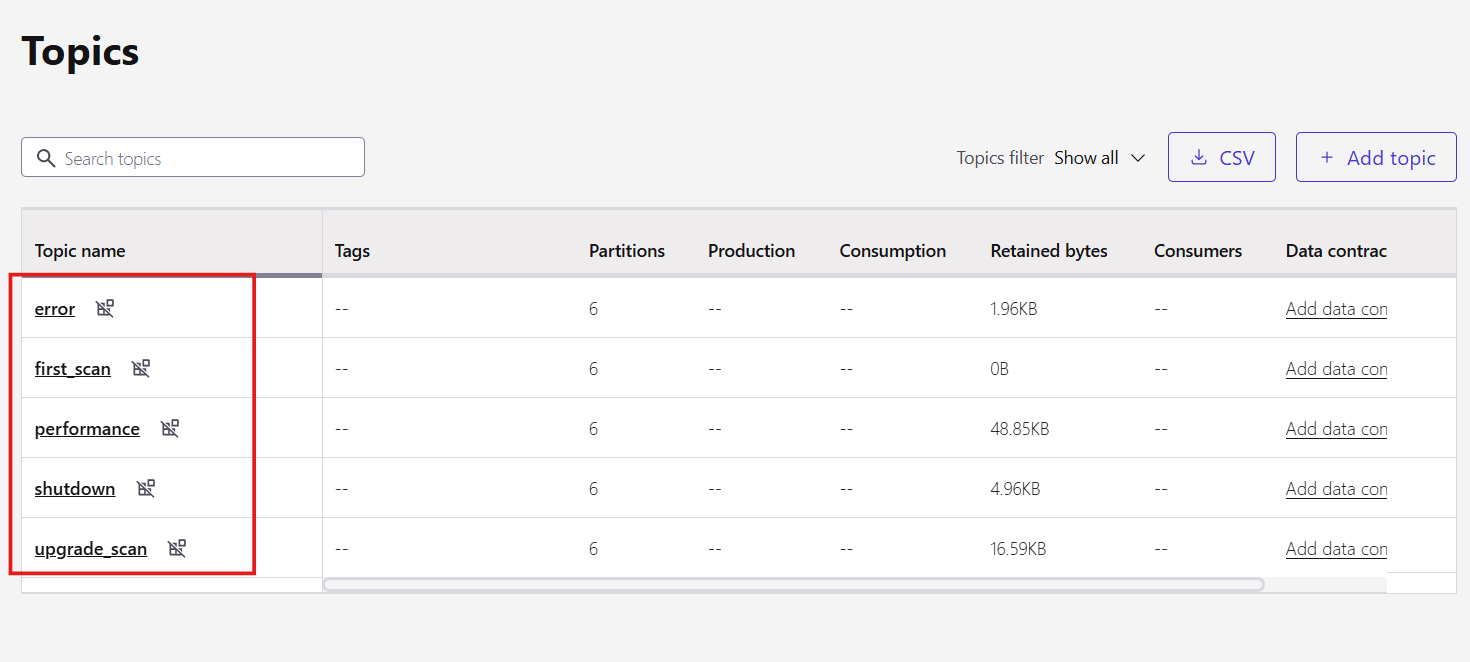
\includegraphics[width=0.9\linewidth]{Images/topic.png}
%     \vspace{10pt}
%     \caption{Topic Config}
%     \label{fig:enter-label}
% \end{figure}
% \noindent Trên Confluent Cloud nhóm đã cài đặt tổng cộng 4 topic cho một cluster phục vụ tương ứng 4 nghiệp vụ khác nhau:
% \begin{itemize}[label=--]
%     \item Performance: Dùng để nhận dữ liệu hiệu suất tài sản từ tool Collector và gửi đến Backend Server.
%     \item First Scan: Dùng để nhận dữ liệu cho các tác vụ quét lần đầu khi triển khai tài sản.
%     \item Upgrade Scan: Dùng để nhận dữ liệu cho các tác vụ quét sau khi nâng cấp, thay thế tài sản.
%     \item Error: Dùng để nhận dữ liệu sự cố, hoặc lỗi của thiết bị. Đối với những lỗi xảy ra nhưng máy tính vẫn hoạt động được (thiếu RAM, thiếu ổ cứng, không có GPU) dữ liệu sẽ gửi qua topic Error. Còn đối với các trường hợp khác khiến máy tắt ngay lập tức hoặc không thể kết nối mạng, nhân viên sử dụng tài sản sẽ báo cáo cho nhân viên IT để tiến hành khắc phục sự cố
% \end{itemize}
% \subsubsection{Cấu hình Topic}
% \noindent Mỗi topic sẽ có các thông tin cấu hình như sau :
% \begin{itemize}[label=--]
%     \item Name: Tên topic
%     \item Partitions: Số lượng partition, nhóm đã cài đặt 6 partition cho mỗi topic, mỗi tầng hoặc mỗi phòng ban của công ty/tổ chức sẽ tương ứng với một partition (có thể mở rộng partition theo như cầu). Mỗi partition sẽ có số lượng offset cực kì lớn.
%     \item Cleanup Policy: Cách dữ liệu được xử lý sau khi đã được tiêu thụ. Ở đây nhóm chọn \textbf{delete} để sau khi tiêu thụ tin nhắn sẽ được xóa sau một khoảng thời gian đã cài đặt trước. Ngược lại có thể chọn \textbf{compact} nếu giữ lại bản ghi mới nhất với cùng key.
%     \item Retention time:  Thời gian lưu giữ bản ghi trên topic (tính bằng milliseconds). Xác định Kafka sẽ giữ dữ liệu bao lâu trước khi xóa, ảnh hưởng đến dung lượng lưu trữ. Nhóm đã cài đặt thời gian là 1 tuần 
%     \item Retention Byte: Dung lượng tối đa mà topic có thể lưu giữ. Nếu đạt đến giới hạn này, Kafka sẽ xóa dữ liệu cũ hơn (nếu cleanup.policy=delete). Ở đây nhóm đã không cài đặt giới hạn số byte cho topic.
%     \item Min Replica: Số replica tối thiểu cần đồng bộ để cho phép ghi. Đảm bảo độ bền dữ liệu. Nếu nhỏ hơn số replica in-sync, producer sẽ gặp lỗi khi ghi từ đó tăng tính an toàn. Nhóm đã cài đặt min replica là 2
%     \item Compression Type: Loại thuật toán nén sử dụng cho dữ liệu gửi lên topic. Giảm dung lượng lưu trữ và băng thông mạng, nhưng có thể làm tăng độ trễ do tốn CPU. Nhóm đã cài đặt là "Producer" tức là cấu hình theo Producer
%     \item Max Message Bytes: Kích thước tối đa của một bản ghi Kafka (message). Nhóm đã cài đặt dung lượng tối đa cho một message là 2MB.

% \end{itemize}
% \subsubsection{Cấu hình Producer}
% \noindent Trong hệ thống quản lý tài sản CNTT thời gian thực, dữ liệu từ các máy trạm người dùng được thu thập bởi một module có tên gọi là Collector. Collector đóng vai trò như một producer gửi thông tin giám sát hiệu suất, phần cứng, phần mềm của máy tính cá nhân đến hệ thống trung tâm thông qua nền tảng Confluent Cloud.\\ \\
% Để kết nối đến Confluent Cloud, Collector cần cấu hình một số thông số bảo mật nhằm đảm bảo kênh truyền dữ liệu được mã hóa và xác thực đầy đủ. Cấu hình Producer như sau:
% \begin{itemize}[label=--]
%     \item \textbf{Bootstrap.servers}: Địa chỉ máy chủ Kafka broker để kết nối ban đầu, sau đó producer sẽ tự động phát hiện các broker khác trong cluster. 
%     Nhóm đã thiết lập đường dẫn là "pkc-l7j7w.asia-east1.gcp.confluent.cloud:9092". Đây là endpoint của Confluent Cloud ở region Asia-East1 (Đài Loan) trên nền tảng GCP.
%     \item \textbf{Security.protocol}: Nhóm đã thiết lập là "SASL\_SSL", tức là Chỉ định sử dụng SASL (Simple Authentication and Security Layer) với SSL để mã hóa kết nối.
%     \item \textbf{SASL Mechanism}: PLAIN , Cơ chế xác thực đơn giản bằng username/password.
%     \item \textbf{SASL Username}: API Key để xác thực với Confluent Cloud.
%     \item \textbf{SASL Password}: API secret tương ứng với key trên.
%     \item \textbf{Client Id}: Định danh duy nhất cho producer, giúp theo dõi và quản lý client.
%     \item \textbf{Retries}: 3 , thử gửi lại tối đa 3 lần khi gặp lỗi mạng.
% \end{itemize}
% \subsubsection{Cấu hình Consumer}
% \noindent Để tiêu thụ dữ liệu từ Kafka trên nền tảng Confluent Cloud, Consumer được thiết lập ở Backend server và được chạy dưới dạng dịch vụ nền (Background Service). Cấu hình Consumer như sau:
% \begin{itemize}[label=--]
%     \item \textbf{BootstrapServers}: Đây là địa chỉ Kafka Broker mà Consumer sẽ kết nối ban đầu. Sau khi kết nối, Consumer sẽ tự động phát hiện các broker khác trong cluster. Nhóm đã cài đặt như ở Producer.
%     \item Các thông số \textbf{Security Protocol}, \textbf{SASL Mechanism} và cả \textbf{Username, password} được cài đặt như ở Producer.
%     \item \textbf{GroupId}: Mỗi Consumer Group có một ID duy nhất để Kafka theo dõi offset (vị trí đọc dữ liệu).
%     \item \textbf{AutoOffsetReset}: Xác định hành vi khi Consumer Group mới hoặc offset không tồn tại. Có hai lựa chọn là Latest (Bắt đầu đọc từ message mới nhất - bỏ qua dữ liệu cũ ) và Earliest (Bắt đầu đọc từ message đầu tiên trong topic), để phù hợp với hệ thống nhóm đã chọn "Latest". Lựa chọn này chỉ quan tâm dữ liệu mới, không cần xử lý dữ liệu cũ. Ngoài ra có thể tránh xử lý lại lượng lớn dữ liệu lịch sử. 
%     \item \textbf{EnableAutoCommit}: Nếu là True, Consumer sẽ tự động commit offset sau khi xử lý message. 
% \end{itemize}

% \subsection{Hiện thực các tính năng}
% \noindent Nhóm tiến hành xây dựng hệ thống web với mục tiêu là cung cấp một giao diện đẹp, trực quan, và dễ sử dụng cho người dùng, đồng thời đáp ứng được các yêu cầu chức năng đã đề cập trước đó.

% \begin{itemize}[label=--]
%     \item Hiện thực tính năng giám sát\\
%     Để truy cập tính năng này, người dùng cần đăng nhập, sau đó bấm vào nút "Bảng giám sát". Giao diện thời gian thực sẽ liên tục cập nhật trạng thái của các máy tính có trong hệ thống, giúp người dùng (nhân viên IT) dễ dàng phát hiện những máy tính cần hỗ trợ (xem thêm ở phụ lục).
%     \begin{figure}[H]
%         \centering
%         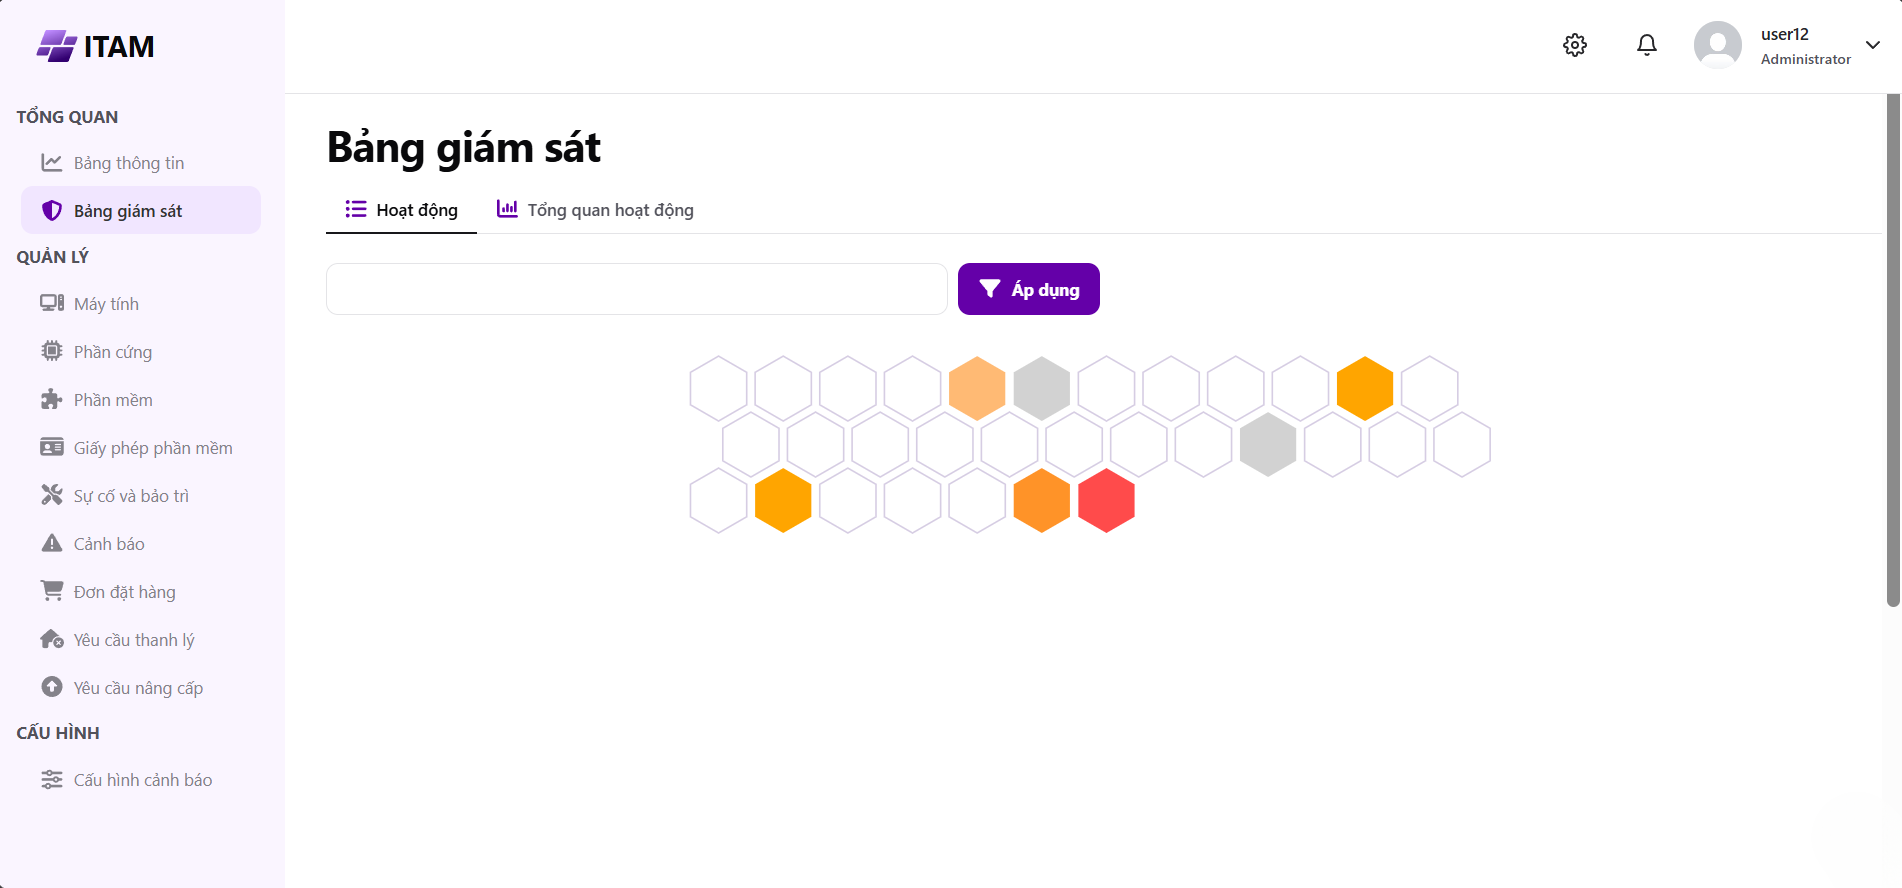
\includegraphics[width=14cm]{Images/C6/UI-Hienthuc/giamsat1.png}
%         \vspace{15pt}
%         \caption{Giao diện hiện thực tính năng Giám sát}
%     \end{figure}

%     \item Hiện thực tính năng quản lý máy tính\\
%     Để truy cập tính năng này, người dùng cần đăng nhập, sau đó bấm vào nút "Máy tính". Ở tính năng này, người dùng có thể thêm thông tin máy tính để quản lý, xem danh sách và chi tiết của máy tính cũng như thông tin vòng đời, hiệu suất, cảnh báo sớm, phần cứng, phần mềm liên quan tới máy tính (xem thêm ở phụ lục).
%     \begin{figure}[H]
%         \centering
%         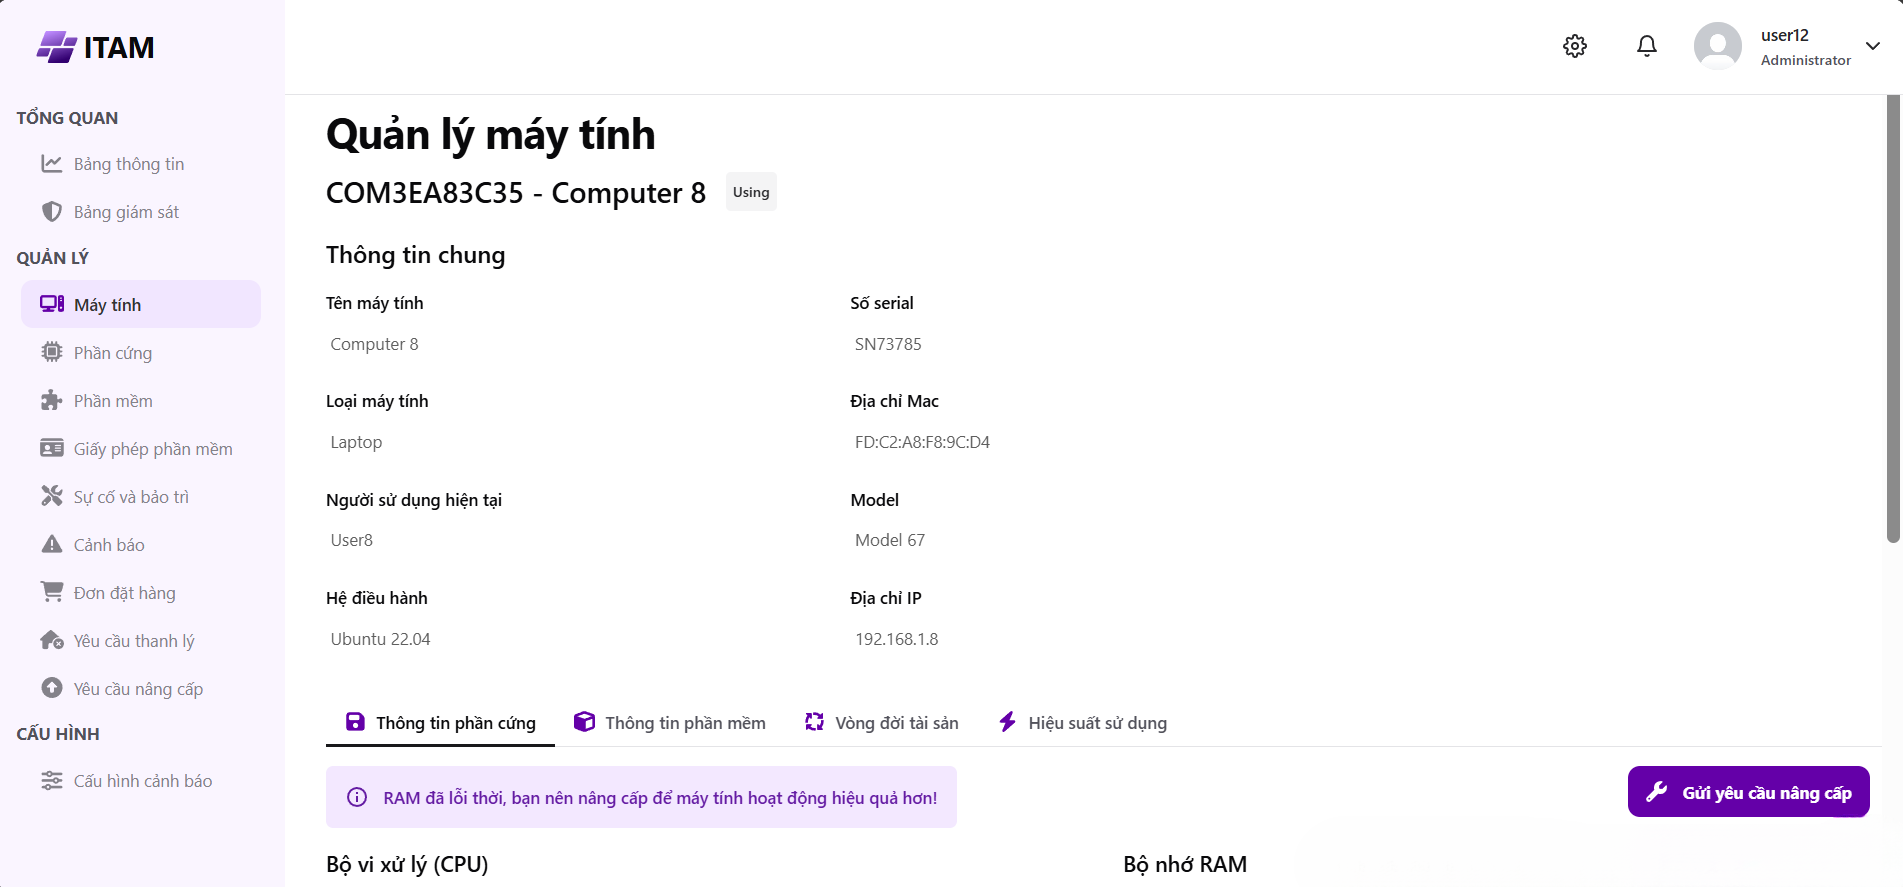
\includegraphics[width=14cm]{Images/C6/UI-Hienthuc/quanlymt1.png}
%         \vspace{15pt}
%         \caption{Giao diện hiện thực tính năng Quản lý máy tính}
%     \end{figure}
%     \begin{figure}[H]
%         \centering
%         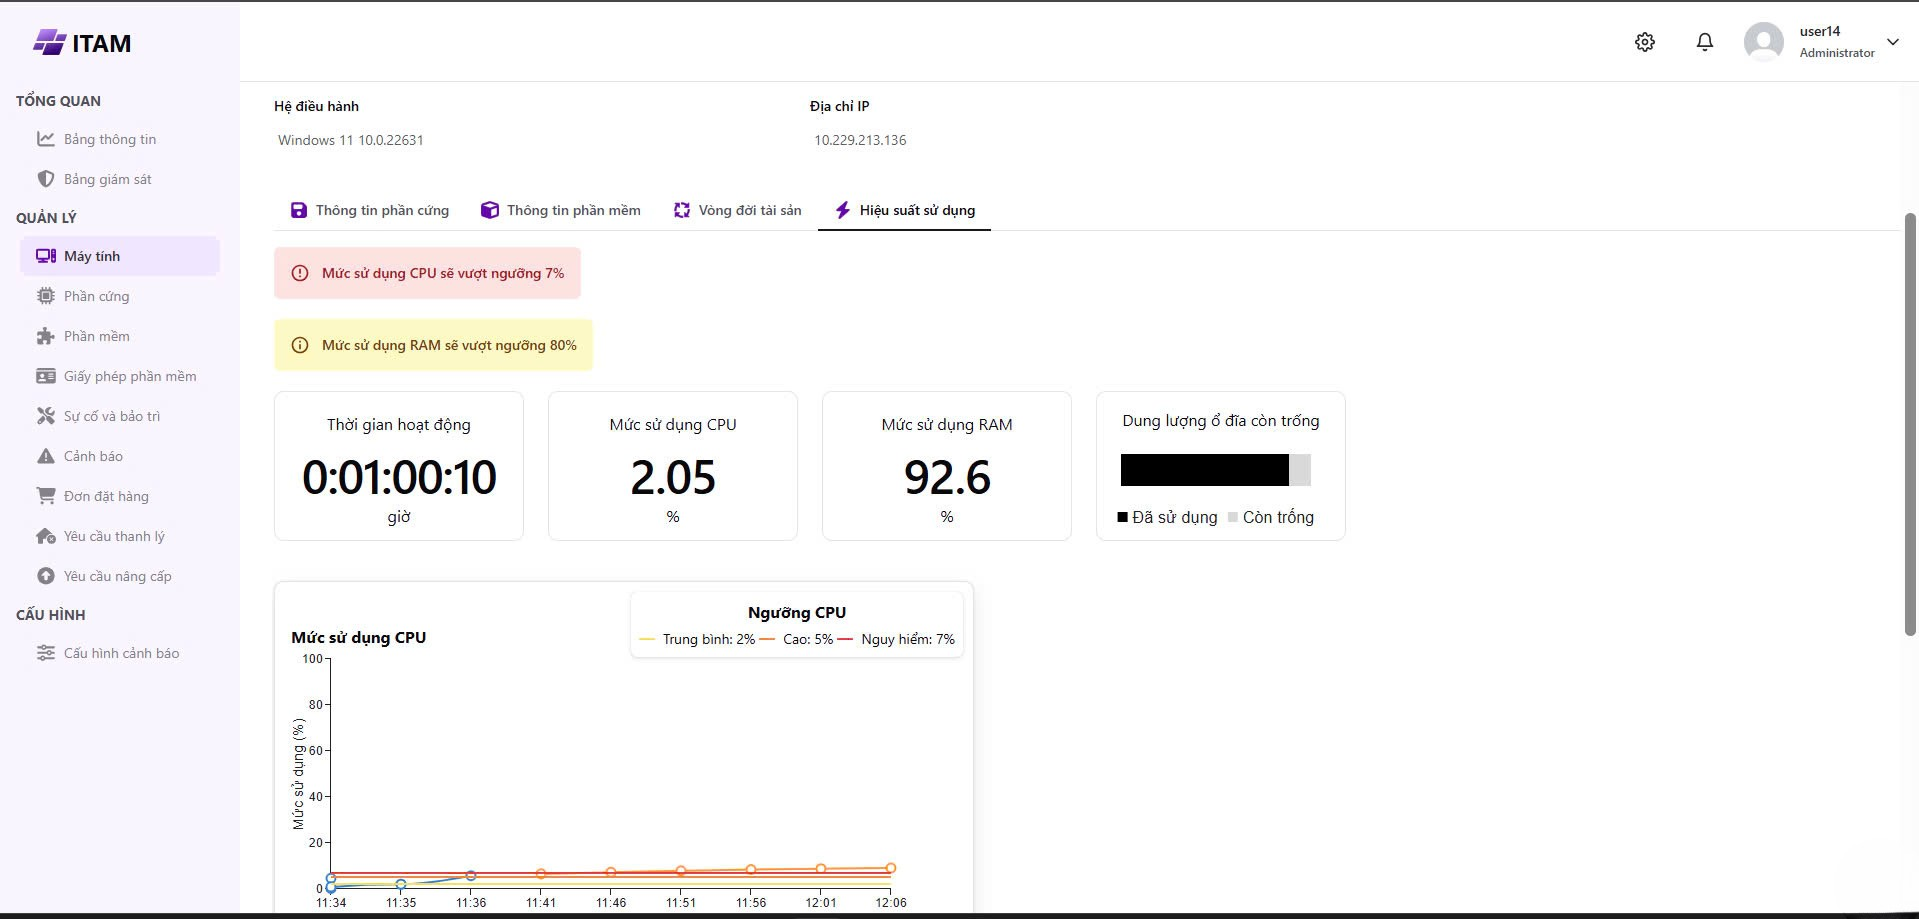
\includegraphics[width=14cm]{Images/C6/UI-Hienthuc/quanlymt3.jpg}
%         \vspace{15pt}
%         \caption{Giao diện hiện thực tính năng Quản lý máy tính - hiệu suất, cảnh báo sớm}
%     \end{figure}

%     \item Hiện thực tính năng Bảng thông tin chung\\
%     Để truy cập tính năng này, người dùng cần đăng nhập, sau đó bấm vào nút "Bảng thông tin". Ở tính năng này, người dùng có thể xem các thông tin chung như tổng giá trị tài sản, tổng yêu cầu nâng cấp bảo trì, đơn đặt hàng (xem thêm ở phụ lục).

%     \item Hiện thực tính năng Quản lý phần cứng, phần mềm\\
%     Để truy cập tính năng này, người dùng cần đăng nhập, sau đó bấm vào nút "Phần cứng" hoặc "Phần mềm". Ở các tính năng này, người dùng có thể xem, chỉnh sửa thông tin về phần cứng, phần mềm, vòng đời của phần cứng, phần mềm và thêm phần cứng, phần mềm vào hệ thống (xem thêm ở phụ lục).

%     \item Hiện thực tính năng Quản lý Giấy phép phần mềm\\
%     Để truy cập tính năng này, người dùng cần đăng nhập, sau đó bấm vào nút "Giấy phép phần mềm". Ở các tính năng này, người dùng có thể xem, chỉnh sửa thông tin giấy phép phần mềm (xem thêm ở phụ lục).

%     \item Hiện thực tính năng Quản lý Sự cố và bảo trì\\
%     Để truy cập tính năng này, người dùng cần đăng nhập, sau đó bấm vào nút "Sự cố và bảo trì". Ở các tính năng này, nhân viên IT có thể xem thông tin sự cố và bảo trì, xác nhận sử lý sự cố và hoàn thành bảo trì (xem thêm ở phụ lục).

%     \item Hiện thực tính năng Quản lý Cảnh báo\\
%     Để truy cập tính năng này, người dùng cần đăng nhập, sau đó bấm vào nút "Cảnh báo". Ở các tính năng này, nhân viên IT có thể dễ dàng xem thông tin của tất cả cảnh báo để có thể ra quyết định xử lý kịp thời (xem thêm ở phụ lục).

%     \item Hiện thực tính năng Quản lý Đơn đặt hàng\\
%     Để truy cập tính năng này, người dùng cần đăng nhập, sau đó bấm vào nút "Đơn đặt hàng". Ở các tính năng này, người quản lý, nhân viên IT có thể xem thông tin đơn hàng. Người quản lý có thể tạo đơn mới hoặc nhập đơn hàng (xem thêm ở phụ lục).

%     \item Hiện thực tính năng Quản lý Yêu cầu nâng cấp, Yêu cầu thanh lý\\
%     Để truy cập tính năng này, người dùng cần đăng nhập, sau đó bấm vào nút "Yêu cầu nâng cấp" hoặc "Yêu cầu thanh lý". Ở các tính năng này, người dùng có thể xem thông tin của tất cả yêu cầu nâng cấp và thanh lý. Người quản lý có thể tiến hành phê duyệt các yêu cầu này (xem thêm ở phụ lục).

%     \item Hiện thực tính năng Cấu hình cảnh báo\\
%     Để truy cập tính năng này, người dùng cần đăng nhập, sau đó bấm vào nút "Cấu hình cảnh báo". Nhân viên IT có thể cấu hình các ngưỡng cảnh báo cho hệ thống (xem thêm ở phụ lục).

%     \item Hiện thực tính năng Báo cáo tổng quan\\
%     Hệ thống còn cung cấp tính năng báo cáo tổng quan như tổng quan về máy tính, phần cứng, phần mềm,... Cung cấp các thông tin tổng quan về số lượng, tình trạng sử dụng, giá trị tài sản,... (xem thêm ở phụ lục).
    
% \end{itemize}

% \subsection{Kiểm thử}
% \noindent Kiểm thử là một giai đoạn quan trọng và không thể thiếu trong quá trình phát triển phần mềm. Nó giúp nhóm phát hiện sớm các lỗi để khắc phục kịp thời, đảm bảo phần mềm hoạt động chính xác, đúng với yêu cầu đặt ra. Dưới đây là kiểm thử cho module giám sát tài sản.
% \subsubsection{Mô tả}
% \noindent Nhóm Giám sát Tài sản tập trung vào việc thu thập và quản lý các thông tin liên quan đến tài sản công nghệ trong hệ thống. Điều này bao gồm việc theo dõi trạng thái, vị trí, tình trạng sử dụng và các thuộc tính khác của tài sản. Mục tiêu chính là giúp tổ chức có cái nhìn toàn diện về tài sản của mình, từ đó tối ưu hóa quản lý và sử dụng.
% \subsubsection{Các bảng dữ liệu liên quan}
% \begin{longtable}{|p{4cm}|p{10cm}|}
%     \caption{Bảng dữ liệu liên quan} \\
%     \hline
%     \textbf{Tên bảng} & \textbf{Mô tả} \\
%     \hline
%     \endfirsthead

%     \hline
%     \textbf{Tên bảng} & \textbf{Mô tả} \\
%     \hline
%     \endhead

%     Asset & Quản lý thông tin chung về tài sản \\
%     \hline
%     Maintenance & Quản lý lịch sử bảo trì của tài sản \\
%     \hline
%     Alert & Ghi nhận các cảnh báo liên quan đến hiệu suất để kịp thời xử lý sự cố. \\
%     \hline
%     AvgPerformance & Lưu trữ dữ liệu hiệu suất trung bình của các thiết bị để phục vụ việc đánh giá và tối ưu sử dụng. \\
%     \hline
%     Lifecycle & Quản lý vòng đời tài sản (Procurement, Implementation, Utilization, Disposal) \\
%     \hline        
% \end{longtable}


% \subsubsection{Các kịch bản kiểm tra}
% \newpage
% \begin{longtable}{
%     |>{\raggedright\arraybackslash}p{0.05\textwidth}
%     |>{\raggedright\arraybackslash}p{0.15\textwidth}
%     |>{\raggedright\arraybackslash}p{0.2\textwidth}
%     |>{\raggedright\arraybackslash}p{0.3\textwidth}
%     |>{\raggedright\arraybackslash}p{0.2\textwidth}|
% }
%     \caption{Các kịch bản kiểm tra} \\
%     \hline
%     \textbf{ID} & \textbf{Testcase} & \textbf{Description} & \textbf{Step} & \textbf{Kết quả} \\
%     \hline
%     % \vspace{0.1pt} A01 &\vspace{0.1pt} Tạo mới tài sản máy tính (vai trò ITStaff, Admin) & \vspace{0.1pt} Người dùng với vai trò ITStaff hoặc Admin tạo mới một tài sản máy tính thông qua giao diện web & 
%     % \begin{itemize}[leftmargin=*,nosep,topsep=0pt,itemsep=0pt]
%     %     \item Log into the website with an Admin or ITStaff account
%     %     \item Click on "Máy tính"
%     %     \item Click on "Thêm máy tính"
%     %     \item Click on "Tên máy tính"
%     %     \item Enter "Test Computer" into "Tên máy tính"
%     %     \item Click on "Loại máy tính"
%     %     \item Enter "Laptop" into "Loại máy tính"
%     %     \item Click on "Model"
%     %     \item Enter "Model 21" into "Model"
%     %     \item Click on "Số serial"
%     %     \item Enter "SN30265" into "Số serial"
%     %     \item Click on "Hệ điều hành"
%     %     \item Enter "Ubuntu 22.04" into "Hệ điều hành"
%     %     \item Click on "Lưu"
%     %     \item Click on "Search..."
%     %     \item Enter "Test Computer" into "Search..."
%     % \end{itemize} &
%     % \begin{itemize}[leftmargin=*,topsep=0pt,itemsep=0pt]
%     %     \item Dữ liệu tài sản được lưu thành công
%     %     \item Hiển thị đúng tài sản khi tìm kiếm
%     % \end{itemize} \\
%     % \hline    
%     \vspace{0.1pt} A01 & \vspace{0.1pt} Kiểm tra quyền hạn tạo tài sản (vai trò Manager) & \vspace{0.1pt} Người dùng với vai trò Manager không được phép tạo tài sản máy tính & 
%     \begin{itemize}[leftmargin=*,topsep=0pt,itemsep=0pt,label=--]
%         \item Log into the website with a Manager account
%         \item Click on "Máy tính"
%     \end{itemize} &
%     \begin{itemize}[leftmargin=*,topsep=0pt,itemsep=0pt,label=--]
%         \item Không hiển thị nút "Thêm máy tính"
%         \item Người dùng không có quyền tạo mới tài sản
%     \end{itemize} \\
%     \hline    
%     \vspace{0.1pt} A02 & \vspace{0.1pt} Cập nhật chi tiết tài sản máy tính & \vspace{0.1pt} Cập nhật thông tin tài sản như tên máy tính, người sử dụng hiện tại, địa chỉ IP & 
%     \begin{itemize}[leftmargin=*,topsep=0pt,itemsep=0pt,label=--]
%         \item Log into the website with an Administrator or ITStaff account
%         \item Click on "Máy tính"
%         \item Click on "COM00659887"
%         \item Click on "editable input"
%         \item Enter "Computer 66" into "editable input"
%         \item Reload
%     \end{itemize} &
%     \begin{itemize}[leftmargin=*,topsep=0pt,itemsep=0pt,label=--]
%         \item Thông tin cập nhật được lưu thành công
%         \item Hiển thị đúng thông tin sau khi reload
%     \end{itemize} \\
%     \hline
%     \vspace{0.1pt} A03 & \vspace{0.1pt} Kiểm tra quyền hạn chỉnh sửa tài sản (vai trò Manager) & \vspace{0.1pt} Người dùng với vai trò Manager không được phép chỉnh sửa tài sản & 
%     \begin{itemize}[leftmargin=*,topsep=0pt,itemsep=0pt,label=--]
%         \item Log into the website with a Manager account
%         \item Click on "Máy tính"
%         \item Click on "COM00659887"
%         \item Click on "Computer 6"
%     \end{itemize} &
%     \begin{itemize}[leftmargin=*,topsep=0pt,itemsep=0pt,label=--]
%         \item Không thể chỉnh sửa các input field
%     \end{itemize} \\
%     \hline    
%     \vspace{0.1pt} A04 & \vspace{0.1pt} Thông tin phần cứng của máy tính & \vspace{0.1pt} Kiểm tra hệ thống hiển thị đúng thông tin phần cứng của máy tính & 
%     \begin{itemize}[leftmargin=*,topsep=0pt,itemsep=0pt,label=--]
%         \item Log into website
%         \item Click on "Máy tính"
%         \item Click on "COM00659887"
%         \item Click on "Thông tin phần cứng"
%     \end{itemize} &
%     \begin{itemize}[leftmargin=*,topsep=0pt,itemsep=0pt,label=--]
%         \item Hiển thị đúng thông tin CPU, RAM, ổ cứng, card mạng, GPU
%     \end{itemize} \\
%     \hline    
%     \vspace{0.1pt} A05 & \vspace{0.1pt} Thông tin phần mềm của máy tính & \vspace{0.1pt} Kiểm tra hệ thống hiển thị đúng danh sách phần mềm đã cài đặt & 
%     \begin{itemize}[leftmargin=*,topsep=0pt,itemsep=0pt,label=--]
%         \item Log into website
%         \item Click on "Máy tính"
%         \item Click on "COM00659887"
%         \item Click on "Thông tin phần mềm"
%     \end{itemize} &
%     \begin{itemize}[leftmargin=*,topsep=0pt,itemsep=0pt,label=--]
%         \item Hiển thị đầy đủ danh sách phần mềm
%         \item Bao gồm tên, phiên bản, nhà phát hành
%     \end{itemize} \\
%     \hline    
%     \vspace{0.1pt} A06 & \vspace{0.1pt} Hiệu suất sử dụng máy tính & \vspace{0.1pt} Kiểm tra tính năng theo dõi hiệu suất hoạt động & 
%     \begin{itemize}[leftmargin=*,topsep=0pt,itemsep=0pt,label=--]
%         \item Log into website
%         \item Click on "Máy tính"
%         \item Click on "COM0AF0C218"
%         \item Click on "Hiệu suất sử dụng"
%     \end{itemize} &
%     \begin{itemize}[leftmargin=*,topsep=0pt,itemsep=0pt,label=--]
%         \item Hiển thị bảng theo dõi hiệu suất CPU, RAM, ổ đĩa
%     \end{itemize} \\
%     \hline
    
%     \vspace{0.1pt} A07 & \vspace{0.1pt} Báo cáo tổng quan máy tính & \vspace{0.1pt} Kiểm tra hệ thống hiển thị báo cáo tổng quan & 
%     \begin{itemize}[leftmargin=*,topsep=0pt,itemsep=0pt,label=--]
%         \item Log into website
%         \item Click on "Máy tính"
%         \item Click on "Báo cáo tổng quan"
%     \end{itemize} & 
%     \begin{itemize}[leftmargin=*,topsep=0pt,itemsep=0pt,label=--]
%         \item Hiển thị số lượng máy tính theo loại
%         \item Hiển thị tình trạng sử dụng
%     \end{itemize} \\
%     \hline    
%     \vspace{0.1pt} A08 & \vspace{0.1pt} Bảng giám sát hoạt động & \vspace{0.1pt} Đảm bảo bảng giám sát hiển thị đúng lỗi và cảnh báo & 
%     \begin{itemize}[leftmargin=*,topsep=0pt,itemsep=0pt,label=--]
%         \item Log into website
%         \item Click on "Bảng giám sát"
%         \item Xem thông tin giám sát của một máy tính
%         \item Kiểm tra cảnh báo hiệu suất
%     \end{itemize} &
%     \begin{itemize}[leftmargin=*,topsep=0pt,itemsep=0pt,label=--]
%         \item Hiển thị realtime các hoạt động
%         \item Cảnh báo khi vượt ngưỡng
%     \end{itemize} \\
%     \hline
%     \vspace{0.1pt} A9 & \vspace{0.1pt} Tổng quan hoạt động tài sản & \vspace{0.1pt} Xác minh giao diện báo cáo tổng hợp tình trạng lỗi & 
%     \begin{itemize}[leftmargin=*,topsep=0pt,itemsep=0pt,label=--]
%         \item Log into website
%         \item Click on "Bảng giám sát"
%         \item Click on "Tổng quan hoạt động"
%     \end{itemize} &
%     \begin{itemize}[leftmargin=*,topsep=0pt,itemsep=0pt,label=--]
%         \item Hiển thị tổng quan tình trạng sử dụng
%         \item Thống kê theo phòng ban, địa điểm
%     \end{itemize} \\
%     \hline
% \end{longtable}
% \noindent Và đó là phần kiểm thử cho module giám sát tài sản của hệ thống. Ngoài ra, nhóm đã thiết kế tổng cộng 6 nhóm testcases tương ứng với các module của hệ thống lần lượt là Quản lý người dùng, Thu thập và quản lý tài sản (Giám sát tài sản), Quản lý vòng đời tài sản; Cấu hình cảnh báo và cảnh báo; Bảo trì và lỗi; Quản lý nhà cung cấp và đơn đặt hàng. Kiểm thử đầy đủ được trình bày tại đây \href{https://docs.google.com/spreadsheets/d/1jniVzouwGwiA-Zut57mP8WkhuAvEHiyQ/edit?usp=sharing&ouid=113898029022770865736&rtpof=true&sd=true}{Link}.
% \subsection{Sử dụng LSTM cho dự đoán hiệu suất sử dụng CPU, RAM}
% \begin{enumerate}
%     \item \textbf{Mô tả dữ liệu}\\ \href{https://drive.google.com/file/d/1M5THsCWqN3WJ1JGntOy3PdtKMNtWeUR1/view?usp=sharing}{Đường link của dữ liệu}\\
%     Dữ liệu được thu thập từ máy của các người dùng khác nhau, liên tục và cách quãng nhau 10 phút. Dữ liệu dùng để huấn luyện có các thông tin như sau:
%     \begin{itemize}[label=--]
%         \item Thông tin CPU: 
%         \begin{itemize}[label=\textbullet]
%             \item Mức độ sử dụng (utilization): Là nhãn trong bài toán dự đoán CPU 
%             \item Số lượng tiến trình đang hoạt động (processes): Góp phần quyết định mức sử dụng CPU và bộ nhớ
%             \item Thời gian hoạt động liên tục (uptime) tính từ thời điểm restart máy đến hiện tại: Càng hoạt động lâu, hệ thống có xu hướng tiêu tốn tài nguyên nhiều hơn
%         \end{itemize}
%         \item Thông tin RAM: tỷ lệ bộ nhớ đang sử dụng (percent).
%         \item Thông tin ổ đĩa: tổng bộ nhớ đã sử dụng (total\_memory\_used), tỷ lệ bộ nhớ đã dùng (percent\_mem\_used).
%         \item Thông tin mạng: tốc độ card mạng (inet\_card\_speed).
%         \item Thông tin hệ thống: thời gian khởi động hệ điều hành (boot\_time), thời gian quét (scantime), vị trí máy (location), và người dùng hiện tại (currentUser). 
%         \item Thông tin về giờ làm việc: thời gian thu thập có phải trong giờ làm việc hay không.
%         \item Ngày trong tuần: ngày thu thập dữ liệu có phải ngày trong tuần không. Nhận biết xu hướng hoạt động theo thời gian làm việc – ví dụ: cao điểm thứ 2-6
%     \end{itemize}
%     Dữ liệu sau khi thu thập được tiền xử lý và lưu vào định dạng CSV để phục vụ cho việc huấn luyện. \\
%     Quá trình tiền xử lý bao gồm: 
%     \begin{itemize}[label=--]
%         \item Xử lý các giá trị bị null và outlier
%         \item Chuyển đổi định dạng thời gian
%         \item Chuẩn hóa dữ liệu đầu vào và đầu ra bằng MinMaxScaler
%     \end{itemize}
%     Sau đó, dữ liệu được gom lại theo chuỗi thời gian, đảm bảo khoảng cách thời gian dữ liệu không quá 20 phút. Sau khi nhóm thành các nhóm nhỏ thì sẽ gộp các chuỗi lại theo CPU riêng và Ram Riêng.
%     \item \textbf{Cấu trúc mô hình LSTM}\\
%     Mô hình dự báo được xây dựng dựa trên kiến trúc Long Short-Term Memory (LSTM) – một biến thể của mạng nơ-ron hồi quy (RNN) chuyên biệt cho xử lý chuỗi thời gian và dữ liệu có tính tuần tự.\\
%     Cấu trúc chi tiết của mô hình như sau:
%     \begin{enumerate}
%         \item \textbf{Lớp LSTM thứ nhất (64 units)}:\\
%         Lớp đầu (return\_sequences=True) trả về chuỗi đầy đủ để lớp thứ hai có thể xử lý thông tin thời gian đa tầng.
%         \begin{itemize}[label=--]
%             \item \textbf{Lựa chọn Activation Functions}: 
%             \begin{itemize}[label=\textbullet]
%                 \item \textbf{tanh} cho trạng thái cell: Giới hạn đầu ra trong khoảng [-1, 1], tránh bùng nổ giá trị.
%                 \item \textbf{sigmoid} cho các cổng (input/forget/output gates): Đưa giá trị về [0, 1], phù hợp cho việc điều khiển tỷ lệ thông tin được giữ/loại bỏ.
%             \end{itemize}
%             \item \textbf{Regularization (L1/L2)}: $l=1e-5$, $l2=1e-4$: Áp dụng regularization để phạt trọng số lớn, ngăn chặn overfitting. L2 (Ridge) thường hiệu quả hơn L1 (Lasso) với RNN do tính chất của dữ liệu chuỗi thời gian.
%             \item \textbf{Batch Normalization (BatchNorm)}: Chuẩn hóa đầu ra sau mỗi lớp LSTM để ổn định phân phối dữ liệu qua các lớp, giảm hiện tượng "internal covariate shift", giúp mô hình hội tụ nhanh hơn.
%             \item \textbf{Dropout 30\%}: Tỷ lệ cao hơn so với thông thường (20\%) do LSTM dễ overfitting với dữ liệu nhỏ. Dropout ngẫu nhiên loại bỏ 30\% units trong quá trình huấn luyện để tăng tính tổng quát.
%         \end{itemize}
%         \item \textbf{Lớp LSTM thứ hai (32 units)}:
%         \begin{itemize}[label=--]
%             \item \textbf{Giảm số units (64 → 32)}: Lớp sau cần ít units hơn do đã trích xuất features quan trọng từ lớp trước. Việc giảm số units giúp giảm tham số, tránh overfitting.
%             \item \textbf{return\_sequences=False}: Chỉ trả về đầu ra cuối cùng (không cần chuỗi) vì bài toán là regression (dự đoán giá trị đơn).
%         \end{itemize}
%         \item \textbf{Lớp Dense trung gian (32 units)}
%         \begin{itemize}[label=--]
%             \item Lớp Dense với ReLU (Rectified Linear Unit) giúp kết hợp phi tuyến tính các features từ LSTM trước khi đưa ra kết quả. ReLU được chọn do tính đơn giản và hiệu quả với dữ liệu không âm.
%             \item Lớp đầu ra (linear): Activation linear phù hợp cho regression vì không giới hạn khoảng giá trị đầu ra.
%         \end{itemize}
%         \item \textbf{Cấu hình huấn luyện}:
%         \begin{itemize}[label=--]
%             \item Adam: Kết hợp ưu điểm của RMSProp và Momentum, tự động điều chỉnh learning rate cho từng trọng số. Hiệu quả với dữ liệu chuỗi thời gian do khả năng xử lý nhiễu.
%             \item Learning rate 0.001: Giá trị phổ biến để cân bằng giữa tốc độ hội tụ và ổn định. Nếu quá lớn, mô hình có thể phân kỳ; quá nhỏ dẫn đến hội tụ chậm.
%             \item Gradient Clipping (clipvalue=0.5): Cắt gradient nếu vượt quá 0.5 để tránh hiện tượng "gradient explosion" (phổ biến ở RNN do tích luỹ gradient qua các bước thời gian).
%             \item Hàm mất mát (loss function): Mean Squared Error (MSE) – phù hợp với bài toán hồi quy liên tục.
%         \end{itemize}
%     \end{enumerate}
%     \item \textbf{Quá trình huấn luyện}\\
%     Mô hình được huấn luyện bằng phương pháp học có giám sát với thông số cấu hình như sau:
%     \begin{itemize}[label=--]
%         \item Số lượng epoch: 100
%         \item Kích thước batch: 32
%         \item Sử dụng kỹ thuật Early Stopping để tự động dừng quá trình huấn luyện khi sai số trên tập kiểm tra không còn giảm sau 10 epoch liên tiếp, đồng thời khôi phục lại trọng số tốt nhất.
%     \end{itemize}
%     Dữ liệu đầu vào có định dạng ba chiều [samples, time steps, features], tương ứng với các đặc trưng đã được chuẩn hóa từ dữ liệu gốc. Kết quả huấn luyện được lưu lại để phục vụ đánh giá và trực quan hóa.
%     \item \textbf{Đánh giá mô hình}:\\
%     Sau quá trình huấn luyện, mô hình được đánh giá trên tập kiểm tra thông qua hàm evaluate() để tính toán giá trị sai số trung bình bình phương (MSE). Ngoài ra, kết quả dự đoán cũng được chuyển đổi ngược trở lại giá trị ban đầu thông qua inverse\_transform nhằm so sánh trực tiếp với giá trị thực tế.
%     Kết quả đạt được:
%     \begin{itemize}[label=--]
%         \item CPU - MAE: 3.73, CPU - RMSE: 5.16
%         \item RAM - MAE: 3.51, RAM - RMSE: 5.73
%         \item CPU Loss: 25.58
%         \item RAM Loss: 32.85
%     \end{itemize}
%     \textbf{Nhận xét}: Kết quả cho thấy mô hình đạt độ chính xác tương đối tốt với cả hai đầu ra là mức sử dụng CPU và RAM. Sai số trung bình tuyệt đối (MAE) đều dưới 4\%, cho thấy dự đoán gần với giá trị thực tế. RMSE và Loss cho RAM cao hơn một chút so với CPU, điều này có thể phản ánh sự dao động lớn hơn hoặc tính khó dự đoán hơn của mức sử dụng RAM theo thời gian. Tuy nhiên, các chỉ số vẫn nằm trong phạm vi chấp nhận được cho các bài toán dự đoán tài nguyên hệ thống trong thực tế.
%     Nhìn chung, mô hình có khả năng dự báo hiệu quả hiệu suất hệ thống trong ngắn hạn, giúp hỗ trợ đưa ra cảnh báo sớm đối với thiết bị.\\ \\
%     Bên cạnh sử dụng mô hình LSTM nhóm cũng đã sử dụng hai mô hình tương tác tốt với dữ liệu tuần tự theo thời gian là RNN (Recurrent Neural Network) thường và GRU (Gated Recurrent Unit).\\
% \noindent Bảng tổng hợp kết quả thu được như sau:
% \begin{longtable}{|p{0.1\textwidth}|p{0.1\textwidth}|p{0.1\textwidth}|p{0.1\textwidth}|p{0.1\textwidth}|p{0.1\textwidth}|p{0.1\textwidth}|}
%     \caption{Tổng hợp kết quả thực nghiệm trên GRU, RNN, LSTM}\\
%     \hline
%     \textbf{Mô hình}  & \textbf{CPU MAE} & \textbf{CPU RMSE} & \textbf{CPU Loss} & \textbf{RAM MAE}& \textbf{RAM RMSE} & \textbf{RAM Loss} \\
%    \hline
%     \textbf{LSTM} & 3.73 & 5.06 & 25.58 & 3.51 & 5.73 & 32.85 \\
%     \hline
%     \textbf{RNN}  & 3.85 & 5.37 & 30.28 & 3.89 & 5.96 & 34.31 \\
%     \hline
%     \textbf{GRU}  & 3.75 & 5.09 & 25.71 & 4.30 & 6.16 & 37.93 \\
%     \hline
% \end{longtable}
% Dựa trên bảng kết quả thực nghiệm, có thể thấy mô hình LSTM đạt hiệu suất tương đối tốt trên hầu hết các chỉ số đánh giá. Cụ thể, LSTM cho giá trị sai số tuyệt đối trung bình (MAE) và sai số bình phương trung bình (RMSE) thấp nhất đối với cả CPU và RAM, lần lượt là CPU MAE = 3.73, CPU RMSE = 5.06, RAM MAE = 3.51, và RAM RMSE = 5.73. Mặc dù GRU có CPU Loss thấp hơn một chút (25.71 so với 25.58 của LSTM), nhưng nhìn chung LSTM vẫn cho thấy sự ổn định và chính xác hơn trên toàn bộ các chỉ số.

% Lý do nhóm lựa chọn LSTM thay vì RNN hoặc GRU là vì LSTM có khả năng ghi nhớ các mối quan hệ dài hạn trong chuỗi thời gian tốt hơn, điều này rất quan trọng trong việc dự đoán hiệu suất tài nguyên như CPU và RAM—vốn phụ thuộc nhiều vào xu hướng sử dụng trong quá khứ. RNN đơn giản thường gặp vấn đề về mất thông tin ở chuỗi dài (vanishing gradient), còn GRU tuy nhẹ hơn nhưng trong thử nghiệm thực tế của nhóm lại cho kết quả kém ổn định hơn so với LSTM. Do đó, LSTM được lựa chọn làm mô hình chính trong hệ thống dự đoán hiệu suất tài sản IT.

% \end{enumerate}

% \subsection{Kết chương}
% Phần kiểm thử được xây dựng trên các kịch bản kiểm tra cụ thể, bám sát các yêu cầu chức năng của từng module. Các trường hợp kiểm thử (testcase) được trình bày rõ ràng với đầu vào, kỳ vọng và kết quả bao gồm các hoạt động như:
% \begin{itemize}[label=--]
%     \item Thêm mới tài sản, phần cứng, phần mềm.
%     \item Cập nhật thông tin và liên kết tài sản với các thực thể liên quan.
%     \item Truy vấn dữ liệu tài sản, bảo trì, lịch sử thay đổi và các thông tin liên quan khác.
%     \item Xóa dữ liệu và kiểm tra liên kết giữa các bảng.
% \end{itemize}
% Nhóm đã thiết kế tổng cộng 6 nhóm kiểm thử, đảm bảo toàn bộ các module chính của hệ thống được kiểm tra đầy đủ và kỹ lưỡng. Điều này không chỉ giúp phát hiện và sửa lỗi trong giai đoạn phát triển mà còn đảm bảo hệ thống hoạt động đúng theo yêu cầu đặt ra. \\ \\
% Ngoài ra, hệ thống còn tích hợp mô hình LSTM (Long Short-Term Memory) nhằm dự đoán hiệu suất sử dụng CPU và RAM của các tài sản theo thời gian. Mô hình được triển khai thông qua một API sử dụng FastAPI, cho phép backend gửi dữ liệu đầu vào và nhận kết quả dự đoán theo yêu cầu.\\ \\
% Nhìn chung, việc hiện thực, kiểm thử và tích hợp trí tuệ nhân tạo đã đặt nền tảng vững chắc cho hệ thống quản lý tài sản CNTT thời gian thực, đảm bảo tính hiệu quả, mở rộng và khả năng thích ứng với các nhu cầu phát triển trong tương lai.
